% This is the Reed College LaTeX thesis template. Most of the work
% for the document class was done by Sam Noble (SN), as well as this
% template. Later comments etc. by Ben Salzberg (BTS). Additional
% restructuring and APA support by Jess Youngberg (JY).
% Your comments and suggestions are more than welcome; please email
% them to cus@reed.edu
%
% See http://web.reed.edu/cis/help/latex.html for help. There are a
% great bunch of help pages there, with notes on
% getting started, bibtex, etc. Go there and read it if you're not
% already familiar with LaTeX.
%
% Any line that starts with a percent symbol is a comment.
% They won't show up in the document, and are useful for notes
% to yourself and explaining commands.
% Commenting also removes a line from the document;
% very handy for troubleshooting problems. -BTS

% As far as I know, this follows the requirements laid out in
% the 2002-2003 Senior Handbook. Ask a librarian to check the
% document before binding. -SN

%%
%% Preamble
%%
% \documentclass{<something>} must begin each LaTeX document
\documentclass[12pt,twoside]{reedthesis}
% Packages are extensions to the basic LaTeX functions. Whatever you
% want to typeset, there is probably a package out there for it.
% Chemistry (chemtex), screenplays, you name it.
% Check out CTAN to see: http://www.ctan.org/
%%
\usepackage{graphicx,latexsym}
\usepackage{amsmath}
\usepackage{amssymb,amsthm}
\usepackage{longtable,booktabs,setspace}
\usepackage{chemarr} %% Useful for one reaction arrow, useless if you're not a chem major
\usepackage[hyphens]{url}
% Added by CII
\usepackage{hyperref}
\usepackage{lmodern}
\usepackage{float}
\floatplacement{figure}{H}
% End of CII addition
\usepackage{rotating}

% Next line commented out by CII
%%% \usepackage{natbib}
% Comment out the natbib line above and uncomment the following two lines to use the new
% biblatex-chicago style, for Chicago A. Also make some changes at the end where the
% bibliography is included.
%\usepackage{biblatex-chicago}
%\bibliography{thesis}


% Added by CII (Thanks, Hadley!)
% Use ref for internal links
\renewcommand{\hyperref}[2][???]{\autoref{#1}}
\def\chapterautorefname{Chapter}
\def\sectionautorefname{Section}
\def\subsectionautorefname{Subsection}
% End of CII addition

% Added by CII
\usepackage{caption}
\captionsetup{width=5in}
% End of CII addition

% \usepackage{times} % other fonts are available like times, bookman, charter, palatino


% To pass between YAML and LaTeX the dollar signs are added by CII
\title{A Musical Stylometry Study on Works by Fanny Hensel and Felix
Mendelssohn}
\author{Emily Palmer}
% The month and year that you submit your FINAL draft TO THE LIBRARY (May or December)
\date{May 2018}
\division{Mathematics and Natural Sciences}
\advisor{Andrew Bray}
\institution{Reed College}
\degree{Bachelor of Arts}
%If you have two advisors for some reason, you can use the following
% Uncommented out by CII
% End of CII addition

%%% Remember to use the correct department!
\department{Mathematics}
% if you're writing a thesis in an interdisciplinary major,
% uncomment the line below and change the text as appropriate.
% check the Senior Handbook if unsure.
%\thedivisionof{The Established Interdisciplinary Committee for}
% if you want the approval page to say "Approved for the Committee",
% uncomment the next line
%\approvedforthe{Committee}

% Added by CII
%%% Copied from knitr
%% maxwidth is the original width if it's less than linewidth
%% otherwise use linewidth (to make sure the graphics do not exceed the margin)
\makeatletter
\def\maxwidth{ %
  \ifdim\Gin@nat@width>\linewidth
    \linewidth
  \else
    \Gin@nat@width
  \fi
}
\makeatother

\renewcommand{\contentsname}{Table of Contents}
% End of CII addition

\setlength{\parskip}{0pt}

% Added by CII

\providecommand{\tightlist}{%
  \setlength{\itemsep}{0pt}\setlength{\parskip}{0pt}}

\Acknowledgements{

}

\Dedication{

}

\Preface{

}

\Abstract{
The use of quantitative methods for attribution of pieces of classical
music to composers is a relatively underexplored field. In theory,
composers leave behind unconscious (or perhaps conscious) signals that
indicate a piece of music as their own. Ideally these signals or
features can be extracted and used to build a model to predict the
composer of a piece of music. For instance, the siblings Fanny Hensel
and Felix Mendelssohn, although very similar in compositional style,
likely have features that distinguish their music. It is speculated that
there are at least six pieces that Fanny wrote that were published by
Felix. This historical setting motivates the construction of a model to
determine which sibling was the true author.

Low level features including frequencies of chords and scale degrees,
were extracted from 31 lieder known to be written by Felix and 35 pieces
known to be written by Fanny. These features were extracted using museR,
an R package written for the purpose of this thesis. Additionally, to
check the validity of features used, 27 solo piano pieces from J.S.
Bach's Well Tempered Clavier were also included in the analysis.
Logistic lasso, \(k-\)nearest neighbors, random forests, naive Bayes,
and linear discriminant analysis were performed on the feature space in
order to classify the pieces. In addition, those same models were fit on
the principal components. The LDA model fit on the principal components
comparing Bach and Mendelssohn resulted in the lowest misclassification
rate (0.049). The logistic lasso model on the principal components
between Felix and Fanny resulted in the lowest misclassification rate
(0.45). Finnaly, each model was used to predict the authorship of the
the six disputed pieces. As misclassification rates were so high on the
models, we cannot trust the predictions for these disputed pieces.
}

	\usepackage{tikz,amsmath,graphicx,}
	\usetikzlibrary{shapes,arrows}
	\newcommand*{\h}{\hspace{5pt}}% for indentation
	\newcommand*{\hh}{\h\h}% double indentation
% End of CII addition
%%
%% End Preamble
%%
%

\usepackage{amsthm}
\newtheorem{theorem}{Theorem}[chapter]
\newtheorem{lemma}{Lemma}[chapter]
\theoremstyle{definition}
\newtheorem{definition}{Definition}[chapter]
\newtheorem{corollary}{Corollary}[chapter]
\newtheorem{proposition}{Proposition}[chapter]
\theoremstyle{definition}
\newtheorem{example}{Example}[chapter]
\theoremstyle{definition}
\newtheorem{exercise}{Exercise}[chapter]
\theoremstyle{remark}
\newtheorem*{remark}{Remark}
\newtheorem*{solution}{Solution}
\begin{document}

% Everything below added by CII
  \maketitle

\frontmatter % this stuff will be roman-numbered
\pagestyle{empty} % this removes page numbers from the frontmatter



  \hypersetup{linkcolor=black}
  \setcounter{tocdepth}{2}
  \tableofcontents

  \listoftables

  \listoffigures
  \begin{abstract}
    The use of quantitative methods for attribution of pieces of classical
    music to composers is a relatively underexplored field. In theory,
    composers leave behind unconscious (or perhaps conscious) signals that
    indicate a piece of music as their own. Ideally these signals or
    features can be extracted and used to build a model to predict the
    composer of a piece of music. For instance, the siblings Fanny Hensel
    and Felix Mendelssohn, although very similar in compositional style,
    likely have features that distinguish their music. It is speculated that
    there are at least six pieces that Fanny wrote that were published by
    Felix. This historical setting motivates the construction of a model to
    determine which sibling was the true author.
    
    Low level features including frequencies of chords and scale degrees,
    were extracted from 31 lieder known to be written by Felix and 35 pieces
    known to be written by Fanny. These features were extracted using museR,
    an R package written for the purpose of this thesis. Additionally, to
    check the validity of features used, 27 solo piano pieces from J.S.
    Bach's Well Tempered Clavier were also included in the analysis.
    Logistic lasso, \(k-\)nearest neighbors, random forests, naive Bayes,
    and linear discriminant analysis were performed on the feature space in
    order to classify the pieces. In addition, those same models were fit on
    the principal components. The LDA model fit on the principal components
    comparing Bach and Mendelssohn resulted in the lowest misclassification
    rate (0.049). The logistic lasso model on the principal components
    between Felix and Fanny resulted in the lowest misclassification rate
    (0.45). Finnaly, each model was used to predict the authorship of the
    the six disputed pieces. As misclassification rates were so high on the
    models, we cannot trust the predictions for these disputed pieces.
  \end{abstract}

\mainmatter % here the regular arabic numbering starts
\pagestyle{fancyplain} % turns page numbering back on

\chapter{}\label{section}

\section{Introduction}\label{introduction}

Treating text or music as data has challenges. Neither data nor music
contains anything immediately analyzable by a computer. With the
increasing availability of the internet and social media data, text
classification has become a promising form of data analysis. While
methods have been developed to attribute authorship of text, such
methods have yet to be thoroughly explored for authorship of classical
music.

Feature extraction is an essential part of text or music classification.
Unlike in other applications where the data initially contains an
informative set of numerical or categorical values, text and music must
first go through a processing stage where features of interest can be
extracted before any models can be fit.

Studies that examine the style of a type of music or composer using
computation are known as musical stylometry studies. A subfield of
musical stylometry is using the examined style to classify composer.
These studies use extracted features to build a model that can classify
a likely composer for that piece of music. For musically trained humans,
classifying composer on their own might be an easy task. Some are able
to automatically distinguish a piece composed by Bach or Mozart either
by listening to a recording or looking at sheet music. Distinguishing
composers by ear becomes more difficult when composers are
contemporaries. Mozart and Salieri might be distinguishable to a more
discerning listener or scholar, but only with some difficulty. When the
identity of the composer is unknwon or disputed, trying to classify the
piece by ear becomes particularly challenging. Examples of disputed
authorship exist throughout music history, most notably in the
Renaissance era and earlier (Brinkman, Shanahan, \& Sapp, n.d.).

In both text and music classification, we must first extract features
from each piece that ideally signal some distinguishable tendency of the
composer.

\section{Brief history of text
classification}\label{brief-history-of-text-classification}

The Federalist Papers were one of the earliest instances of text
classification for determining authorship (Mosteller \& Wallace, 1964).
These famous 18th century documents were written under the pen name
`Publius'. Several of these disputed papers are attributed to either
James Madison or Alexander Hamilton. Neither of them ever admitted
authorship, as some of the writings were contradictory to their later
political positions (Adair, 1944). Prior to quantitative analysis,
historians had often examined the papers using styles of previously
known writings of Madison and Hamilton. Their analysis was often
partially based on the content of the papers, for example the existence
of citing English history is a trait more common to Hamilton (Ford \&
Bourne, 1897).

In contrast, Mosteller and Wallace (1964) used the frequency of words
such as `and', `by', `from', and `upon', to fit a classifier that was
trained on the writings on a set of known writings by each author. These
unconscious indicators were able to differentiate between the two
writers, and the model was able to identify the likely author of the
disputed paper.

\section{Feature selection}\label{feature-selection}

Text analysis, such as in the Federalist Papers, is accomplished by
reading one word after another. This often results in a vector where
each entry is a word. Frequencies of word count for example, can easily
be done by counting all instances of word occurrence in the word vector.
Information in a piece of music, however, is read in a variety of ways.
It can be read left to right note by note, but it can also be read
vertically as the harmony, or the notes played together. In a piece with
several instruments, both these processes happen at the same time for
each instrument. There are also aspects that take place over large
sections, such as phrasing, or cadential patterns. There are rules of
counterpoint that are followed throughout the entire piece. Thus we need
to find features that can be measured for each piece, or perhaps each
measure or instrument, that can describe a certain piece of music.
Ideally, these features are not measuring certain rules and practices of
classical music, but instead the creativeness and individuality of a
composer. As there are many different aspects of a piece, melodic
changes, harmonies, etc., one can end up with many features to describe
one piece. It is possible that the number of features \((p)\) can be
greater than the sample size \((n)\), or that many features encode
essentially the same thing. We thus need to figure a clever way to
decrease our feature space. This can happen in choosing what features we
want to use to model, or by using a dimension reduction technique such
as principal components analysis.

Most musical stylometry literature has focused on composers in the
Renaissance (1400-1600), Baroque (1600-1750), and Classical (1730-1820)
eras. The Mendelssohns were composing in the Romantic era (1780-1910).
The focus of the literature may have been because composers in earlier
eras followed rules of counterpoint more exactly, or perhaps had less
``expressive'' allowances for their composing, thus making it easier to
define and extract features. There are also more pieces with doubtful
authorship in those eras. In addition, Computer Assisted Research in the
Humanities (CCARH) (C. S. Sapp, n.d.) has a large corpus of encoded
music from these times. As will be described later, the initial step of
coding the music is the most time consuming; having music in a format
immediately conducive to analysis is very helpful.

\section{A Very Short Introduction to Music
Theory}\label{a-very-short-introduction-to-music-theory}

Western sheet music is presented on a five line staff, where the
position on the staff defines its sound. The sound of a note depends on
its pitch, which is a specific vibration of sound waves at a certain
frequency. Notes are in the set
\(note \in \{A\flat,A,A\sharp,B\flat,B,B\sharp,C\flat,C,C\sharp,D\flat,D,D\sharp,E\flat,E,E\sharp,F\flat,F,F\sharp,G\flat,G\,G\sharp\}\),
and the value can be changed up or down a half step by adding a sharp or
flat. To remove sharps of flats, a natural sign is used (\(\natural\))
There also exist double flats and double sharps. Some notes can be
written differently, but sound the same, such as \(F\flat\) and \(E\).
These are known as enharmonics. Of the above possible notes, there are
only twelve distinct notes (i.e.~only twelve half steps in the western
scale). The \emph{key signature} of the piece indicates how many sharps
or flats are normal for the piece. Each key is made up of seven
different notes. A piece's key can be major or minor, although the piece
can internally modulate between the two. The \emph{scale degree} of a
note depends on how many notes it is away from the note that represents
the key of the piece. The \emph{time signature} of a piece determines
the number of beats that are in each measure. The vertical distance
between notes (also known as an \emph{interval}) depends on how many
half steps occur between two notes. \emph{Melodic intervals} are defined
as the number of half steps between two adjacent notes. \emph{Harmonic
intervals} are defined as the number of half steps between notes played
at the same time. \emph{Chords} occur when there are more than two notes
being played simultaneously. The type of chord is determined by the
harmonic intervals it contains. Cadences are a type of chord
progression, usually occurring at the end of a phrase and especially at
the end of a piece. Intervals and chords can be either \emph{dissonant}
or \emph{consonant}. Consonant intervals sound nice to our ears, whereas
dissonant intervals add a sense of tension or unease, which is used to
shape the feel of the music. In addition, chords and intervals can be
minor or major. Minor intervals feel ``sad'', whereas major intervals
feel ``happy''. These are also known as sonorities, and are divided into
three types: perfect intervals (1, 4, 5, and 8), imperfect intervals (3
and 6), and dissonant intervals (2 and 7). There are some rules, known
as counterpoint, that most composers follow to some extent. These were
followed more strictly in the Baroque era than the Romantic era. First
species counterpoint is a type of counterpoint that dictates there are
no parallel octaves, fourths or fifths. Another rule is that when
changing from one perfect consonance to another, the notes must proceed
in contrary or oblique motion (Laitz, 2012).

\section{Musical features}\label{musical-features}

Features calculated from music often closely follow music theory. In
addition to deciding the features, there is also the decision of the
scope at which those features take place. The features can be for a
given instrument, the entire piece, or each measure. Windowing
techniques can be used where a ``window'' is created over a given number
of bars or notes, and shifts across the whole piece. For each window, a
feature is recorded. These can be overlapping windows by creating an
``offset'' of a number of beats or notes. Windowing produces more data,
as instead of one feature for each piece, there is a feature for each
window. Backer et.al used windowing techniques in a musical stylometry
study on Bach and his contemporaries. They also used overlapping
windowing over each entire composition to produce more data, using
window of 30 bars to create a high enough number of fragments per piece
and a low enough variance of the feature values between fragments
(Backer \& Kranenburg, 2005).

Musical features are often thought about as either high level or low
level. While the exact definition of each often varies, low level is
often understood to be features such as note frequency, etc. High level
features are more about a broader sense of the piece, including chord
progressions, etc. High level features are often what music experts use
in their analysis, whereas low-level features are more easily extracted
and analyzed by computer. High level features often depend on the
context of where the feature was extracted from. For example, cadences
and modulations (brief changes in key) throughout the piece are easily
found when a human analyzes a piece of music, but are very hard to
generalize as a feature. If one wants to use high-level features, they
would first have to train the feature to see if it was performing
accurately. For this reason, this paper focuses only on low level
features, or features that are context independent.

\section{Background on Variable and Feature
Selection}\label{background-on-variable-and-feature-selection}

Before analysis is done or models are fit, numerous features are often
extracted from the music without knowing a priori which ones will be
helpful in identifying a composer's style. Especially in research
regarding text categorization, data sets have enormous numbers of
variables. We use ``feature'' and ``variable'' interchangeably, with the
exception when features are created from variables, and the distinction
will be made in that case (Guyon \& Elisseeff, 2003). Fitting models
with all of the features that are available can often lead to
overfitting of the model. There are three main ways to deal with this
problem: subset selection, shrinkage models, and dimensionality
reduction. This section gives a broad overview of options for features
selection. The methods used in this thesis will be described in further
detail in chapter 4.

Subset selection methods choose which features to use in a model. There
are many ways to do this and existing feature selection algorithms can
help with this process. One idea to see which features are best for the
model is to look at all possible subsets of the variables and see which
model performs best. All possible subsets of variables is \(2^p-1\),
where \(p\) is the number of features. For large \(p\), this is often
computationally impossible. Instead of fitting all possible subsets,
stepwise selection strategies like forward selection and backward
selection can be used.

Subset selection methods often use some sort of variable ranking tool to
determine which variables are useful to include in the best subset.
Variable ranking uses a score function to assign a score to each
possible variable. It is tempting to only include variables that have a
high score. However, this possibly leads to redundancy. In addition,
variables that are not important by themselves can have a significant
performance improvement when considered with other variables. Single
variable classifiers rank the variable according to its individual
predictive power. The predictive power can be measured in terms of error
rate, or using the false positive or false negative rate. This
classifier cannot distinguish variables that perfectly separate the
data.

Shrinkage methods, in contrast, use all \(p\) features and constrain or
shrink coefficients towards zero instead of choosing a subset of the
features. Ideally, coefficients of features that are not as useful for
the model will be shrunk towards zero, so they do not have a large
effect on the model. Constraining features in this way often leads to a
reduction in variance of the estimates. The most common shrinkage
methods are ridge and lasso (Hoerl, 1959)(Tibshirani, 1996).

Both shrinkage methods and subset selection use the original variables
to fit models. Dimension reduction methods transform the features space,
and then fit models on the transformed variables. It is commonly used to
attempt to encode enough of the information given in the original
features in a smaller-dimensional space. This results in feature
creation; using the recorded variables to create new features to fit the
model on. Common dimension reduction techniques include principal
components analysis (PCA) and linear discriminant analysis (LDA) (Ye,
Janardan, \& Li, 2005). Feature creation aims to achieve a good
reconstruction of the data and to make succesful predictuions using the
constucted features.

Once we have a model, we often want to know how ``good'' it is. For
classification models, we often use the misclassification rate. To
calculate this, we withhold a sample of our data as a testing set. We
then fit the model on the training set, and then use the fitted model to
predict classes on the testing set. The misclassification rate is then
computed as the number of pieces in the testing set that were
incorrectly classified divided by the total number of pieces. Cross
validation involves fitting a model on a training set, and then using
the fitted model to predict the responses in the testing set. In
particular, \(k\)-fold cross validation involves splitting the data set
into \(k\) different parts of equal size, and fitting a model on the the
data set with one of the \(k\) parts withheld. The model is then tested
on the withheld data. This is useful for model selection and determining
the accuracy of the model. In this paper, as is common, we use
\(k = 5\). This results in a predicted misclassification rate with lower
variance that other crossvalidation methods such as leave-one-out-error
and validation sets.

\section{Previous research}\label{previous-research}

There have been numerous other applications of machine learning to
music. These include many studies that are not specifically identifying
a composer from sheet music. For example, a previous study used machine
learning trained on a composer's music to have the computer learn the
style and compose a piece in a similar style. (Papadopoulos \& Wiggins,
n.d.)

Musical stylometry has focused on two types of data: audio and sheet
music. This analysis uses data in the form of sheet music. To predict a
composer, a training data set of pieces of known composer is needed.
Then a model can be fit to a testing data set to predict composer. If
the fitted model shows good predictions, that model can be applied on
the pieces of unknown authorship. Musical stylometry can resolve
disputed authorship and detect distinguishing musical styles of
composer, even if there are no disputed pieces. Musical stylometry can
also look at the development of a composers musical style over time.

This paper draws its inspiration from four different studies that have
classified composers by extracting features from sheet music. Initial
studies in the 1970's started looking at ways to represent music in a
way that could analyzed by computers. Recently, several previous papers
have focused on Josquin des Prez. This is likely due to the fact that
there is a large training and testing data set available in easily
analyzable format provided by the Josquin Research Project (``The
josquin research project,'' n.d.). In addition there are a number of
pieces of disputed authorship that have been attributed to him.

Work by Brinkman et al. (Brinkman et al., n.d.) used machine learning to
evaluate attribution of compositions by Josquin des Prez. They first
compared music of Josquin to JS Bach's four part chorales. Many
listeners could easily distinguish these two composers as they were
separated by two centuries. They also compared Josquin to composers
closer in time and style: Ockeghem and Du Fay, who are only one or two
generations separated. These composers could likely be differentiated by
experienced listeners of Renaissance music. Finally they compared
Josquin's to his contemporaries: de Orto and La Rue.

Work by Backer et. al. looked at differences in style between J.S. Bach,
Telemann, Handel, Haydn and Mozart and then examined a disputed piece:
BWV 534 which is believed to be composed by either J.S. Bach, J.L.
Krebs, or W.F. Bach (J.S. Bach's son) (Backer \& Kranenburg, 2005).

The following two studies do not try to identify composers of unknown
works, but instead try to extract features that can seperate differences
in style, and also fit classifiers that can correctly assign composers
based on their style.

Crerar used incipits from Vivaldi, Correlli, and Valentini, who could
have been a student of Correlli. They used low level features,
especially looking at intervalic movement. They also compared Bach,
Haydn, and Mozart (Crerar, 1985).

Mearns et al. extracted high level musical features on J.S. Bach,
Buxtehude, Ruggero, Vivaldi, Monteverdi, Corelli, and Frescobaldi. The
idea was that they all adhered to the laws of counterpoint, and that
they possibly still had distinct uses of the counterpoint. They used
pieces across instrumental genres with the idea that stylistic
counterpoint would remain constant across compositional type (Mearns,
Tidhar, \& Dixon, 2010).

\section{Previous choices of features in
applications}\label{previous-choices-of-features-in-applications}

Deciding on and extracting features is the first step in analyzing
music. Depending on the characteristics of the composer and time period,
different features are useful. Often features are extracted en masse and
then work is done later to determine which features are important or
useful in identifying style.

In addition to deciding which features to use, one must also determine
the scale at which the features should exist. There can be features for
a given instrument, the entire piece, or each measure. Windowing
techniques can be used where a window is created over a given number of
bars or notes and the window moves through the whole piece. A feature is
extracted and recorded for each window. Windows can be made to overlap
by using an offset of a number of beats or notes. Windowing thus
produces more data as there is a feature for each window instead of for
the whole piece. There can thus be tens of windows in each piece.

Common types of features in music analysis include low level features of
frequencies of notes, chords, etc. Also common are features that look at
the fraction of the score that consisted of dissonant sororities, as
well as the fraction of bars that begin with a dissonant sonority. Other
features include the type of intervals or consonances present in a
piece: perfect consonance, imperfect consonances, and dissonance. In
polyphonic pieces, the four types of motion, (parallel, similar,
oblique, and contrary) can also be used as features. Crerar (Crerar,
1985) used pitch frequencies, after standardizing all pieces by
transposing to the key of C, the first melodic interval of the piece,
and note transition counts. Mearns used types of motion and consonances
as features (Mearns et al., 2010).

Features measuring stability are also popular. Stability can be measured
for rhythmic changes or harmonic changes. Stability is computed by
dividing the standard deviation of the lengths of the rhythm or note by
the mean length of the notes. It is normalized in this way to be
comparable over differing time signatures. Backer and Kranenburg.
(Backer \& Kranenburg, 2005). chose to extract twenty features that
include frequencies of intervals, and measures of stability, and
entropy. The entropy of the probability of occurrence chords was
measured in two different ways, defining chords to be the same no matter
what scale degree they are on, and distinguishing chords differently
depending on scale degree. Next, they the calculated average number of
active voices at one time, a measure of the voice density of the piece.
Then for every interval, the duration of that interval was divided by
the total duration of all intervals. Next, the total duration of
parallel thirds, fourths, and sixths divided by the total duration of
all intervals was measured. Finally, a measure of suspensions was
calculated.

Brinkman et.al (Brinkman et al., n.d.) used both high-level and
low-level features. The high-level features were 9-8 suspensions,
oblique motion, contrary motion, similar motion and parallel motion. The
low-level features were average melodic entropy, normalized pairwise
variability index, and note-to-note transition probabilities.

Other features that can be helpful for distinguishing Renaissance and
Baroque composers look specifically at differences in counterpoint.
Since most composers in that era generally followed the rules of
counterpoint, these features are created to try to detect specific
identifiable uses of counterpoint. These features include counterpoint
movement types, dissonance distributions, parallel intervals of each
kind, and vertical interval distributions. Mearns et al. (Mearns et al.,
2010) calculated intervals for every subsequent pitch in each part. A
weighted count of each interval was stored. The counts were weighted
according to duration to account for the perception of use. The count
vector was then normalized to account for the weighted interval content
of the score. For movement types, Mearns et al. used ideas based on the
rules of first species counterpoint. (Similar, oblique, parallel, and
contrary). It does not make musical sense to compare every single
adjacent group of notes as many of the note groups occurring at
fractional metrical positions consist of notes held from the previous
note group with the addition of a passing or neighbor note in another
voice or voices. For this reason, only notes that occur at strong
metrical positions, in this case on each beat of the bar, are used for
contrapuntal evaluation. This is a relatively simplistic method of
choosing structurally important notes. In Bach, for example, the
majority of voice progressions take place at a closer level. The
features measuring counterpoint rules include the nature of the approach
to a perfect consonance, whether a dissonance is properly prepared
(i.e.~preceded by a consonant interval containing the same note which
then becomes dissonant), whether a dissonance is correctly resolved
downwards by step, details of parallel intervals, and the overall
distribution of contrapuntal movements (oblique / contrary / similar /
parallel / other). A feature for total vertical interval count is also
used.

\section{Previous modeling and results in
applications}\label{previous-modeling-and-results-in-applications}

Most of the previous research has included some kind of feature
selection. Usually features are extracted before any analysis is done,
and we don't know beforehand which features are distinguishing.

A modification of a forward selection (Floating Forward Selection)
(Pudil, Novovičová, \& Kittler, 1994) was used in Backer's (2005) study
to extract features in order to identify distinguishing style between
Bach, Handel, Telemann, Mozart, and Haydn, and then subsequently
classify the authorship of BWV 535. Each composer was compared via
creating bivariate comparisons of all possible class arrangements, ie
(Bach)(Handel), (Bach)(Handel,Telemann), etc. The algorithm extracted
features for each class arrangement that best distinguished the groups.
A \(k\)-nearest neighbors classifier was fit using the features that the
subset selection algorithm found useful. The model was successful in
comparing Bach and others as well as each individual composer. The
\(k\)-nearest neighbor classifier resulted in a leave-one-out-error of
between 5\% and 9\%, for most class arrangements, and 24.3\% between
Hayden and Mozart, Decision trees were also used to interpret the
features used in decision making of the different class arrangements.
The decision trees used between 2 and 4 features depending on which
class comparison was being analyzed. It resulted in a max of one
classification error. To determine authorship of BWV 535, quadratic
Bayesian classifier was trained to distinguish J.S. Bach, W.F. Bach and
J.L Krebs. They again compare every possible class arrangement as
potential composers. Their results showed that BWV 535 was likely
composed by either W.F. Bach and his pupil, J.L. Krebs.

Principal components analysis (PCA) was used for dimension reduction for
subsequent analysis on the music Josquin and his contemporaries.
(Brinkman et al., n.d.) Binary comparisons were used to compare
composers. Although only two principal components accounted for most of
the variance, in the comparison between Bach and Josquin, five principal
components were used to account for more variance (85\%). Between
Josquin and his contemporaries, 27 principal components were used to
account for 85\% of the variance. This resulted in a relatively clear
separation between Bach and Josquin when visualized on their first two
principal components. Between Josquin and each of his contemporaries,
the principal components did not have as much of an obvious separation.
The transformed features from principal components analysis were used to
train a classifier. First, a \(k-\)nearest neighbor classifier was used
with \(k = 6\). The training set consisted of 80\% of the data, with
20\% withheld as a testing set. The model correctly predicted pieces by
de Orto 38.9\% of the time, Josquin 60.6\%, and La Rue, 80.6\% Next,
they trained a support vector machine classifier, which preformed
similarly to the \(k-\)nearest neighbor classifier.

Mearns fit a classifier using a WEKA algorithm, as well as Naive Bayes
and a Decision Tree was created that correctly predicted the composer
2/3 of the time (Mearns et al., 2010).

Crerar took a different approach, and instead of trying to fit a model
that would classify composers, performed a chi-squared test to see if
the features of the composers were in fact different. This would imply
that the composers had different styles that could be distinguished
using the features in the paper. The probability of the chi-squared
values occurring were all less than 0.05, and thus the composers do
indeed have different styles (Crerar, 1985).

\section{Fanny and Felix Mendelssohn}\label{fanny-and-felix-mendelssohn}

Most musical stylometry analysis has focused on music of the Renaissance
and Baroque period, as there are more questions of authorship in that
period. As the Romantic period is much more modern in comparison, there
are many more surviving records of original manuscripts that include the
composer.

Felix Mendelssohn, often considered a prodigy akin to Mozart, was a
prolific composer. Before he was fourteen years old, he had already
written over 100 compositions. His lesser known sister Fanny Hensel née
Mendelssohn was also a composer of incredible skill. The two were very
close, for many years training and studying together. In their early
education living in Berlin, Felix and Fanny received the same musical
education. In their younger years, they were both instructed in piano by
Madam Bigot, a famous pianist esteemed by Haydn and Beethoven. Beginning
in 1818, Carl Friedrich Zelter, a somewhat removed student of Bach and
the most influential Berlin musician of the time, began to teach them
both composition. In addition to music, the children were tutored by
some of the finest scholars in Berlin in subjects such as languages,
history, and drawing. Goethe himself claimed that Fanny was ``as gifted
as Felix'' (Tillard, 1996).

As Fanny grew up, her father started implying that she should focus her
energy on the domestic sphere of her life. While the fact that she never
became a world famous composer and performer is often attributed to the
gender politics of her time, it is also likely due to her high class
(Reich, 1991). Since the family had recently converted from Judaism to
Christianity, and considering the anti-Semitic feelings of the time, the
family did not want any other unusual characteristic such as a
professional female composer to set them further apart from ``polite''
society.

Most of Fanny's available work are \emph{lieder}, short pieces of voice
accompanied by piano. They were accepted at the time as the more
feminine, domestic compositions, acceptable for women to compose. Her
brother moved on to more elaborate compositions such as operas,
orchestral concertos and symphonies. Her father pressured Fanny to
remain composing lieder (Todd, 2003).
\begin{quote}
``Music will perhaps become his profession, while for you it can and
must only be an ornament, never the root of your being and doing. We may
therefore pardon him some ambition and desire to be acknowledged in a
pursuit which appears very important to him,\ldots{} while it does you
credit that you have always shown yourself good and sensible in these
matters; \ldots{} Remain true to these sentiments and to this line of
conduct; they are feminine, and only what is truly feminine is an
ornament to your sex.''
\end{quote}
Throughout their lives, Felix and Fanny maintained contact through
letters until Fanny's death in 1847 and Felix's death shortly
thereafter. These letters contain many instances of Felix asking for
advice on his compositions.

Unlike Felix who conducted and performed piano and organ in some of
Berlin's most esteemed concert halls, most of Fanny's performances were
private, only performed in small circles of her friends and family at
intimate parties. Similarly, although she was quite a prolific composer,
under recommendation of her father Abraham Mendelssohn, and to a lesser
extent Felix, Fanny did not publish her work until later in her life. In
1846 after her father's death and though her brother initially
disapproved, she published her first collection of lieder. Many of
Fanny's unpublished notebooks are in private collections and are
inaccessible for study.

However, it is widely speculated that some of Fanny's work was published
under her brother's name, especially three pieces each in his Op 8 and 9
lieder. Famously, when Felix met the Queen of England, she sang Felix's
lied ``Italien'', and Felix had to admit that in fact, it was his sister
that had written it. In a letter to Felix, Fanny admits:
\begin{quote}
``I have just recently received a letter from Vienna, which contained
basically nothing but the question of whether ``On Wings of Song'' was
by me, and that I should really send a list of things that are running
about in the world disguised, it seems that they aren't clever enough
themselves to separate the wheat from the chaff.'' (Mace, 2013)
\end{quote}
As she never made such a list, we are left to wonder if there are any
other pieces of hers that have been published under her brothers name
and reputation. It is suspected that most of Fanny's friends and family
would have known at the time that she had composed the pieces published
by Felix, as they would have heard her play those pieces at home and for
private audiences. An article written in 1830 in the Harmonicon, an
influential music journal in London, mentioned that not all the lieder
in Felix's collection were written by him. The article also praises the
work of Fanny, albeit in an odd way likely due to the time of
publication.
\begin{quote}
``I possess twelve published songs under Mr.~Mendelssohn's name, which
he wrote when a boy of fifteen. One of these appears in the musical
annual, ``Apollo's Gift,'' and deserves all the praise you have in your
review bestowed on it. But the whole of the twelve are not by him: three
of the best are by his sister, a young lady of great talents and
accomplishments. I cannot refrain from mentioning Miss Mendelsshon's
name in connexion with these songs, more particularly when I see so many
ladies without one atom of genius, coming forward to the public with
their musical crudities, and, because these are printed, holding up
their heads as if they were finished musicians. Miss Mendelssohn is a
first-rate piano-forte player, of which you may form some idea when I
mention that she can express the varied beauties of Beethoven's
extraordinary trio in Bb. She has not the wild energy of her brother;
but possesses sufficient power and nerve for the accurate performance of
Beethoven's music. She is no superficial musician; she has studied the
science deeply, and writes with the freedom of a master. Her songs are
distinguished by tenderness, warmth, and originality: some which I heard
were exquisite.''(Ayrton, 1830)
\end{quote}
This project will use lieder of Fanny and Felix Mendelssohn in attempts
to train a classifier to analyze the six disputed pieces. Most of the
available work by Fanny are lieder. Felix also composed a good number of
lieder. We will see if there is a determinable difference in style of
these siblings who grew up very close and received mostly the same
musical education. All other previous composership studies cannot be
adjusted for training and upbringing, so it might be challenging to
detect a difference.

\chapter{About the data and conversion
process}\label{about-the-data-and-conversion-process}

\section{Pieces used}\label{pieces-used}

The majority of the pieces used in this paper were lieder of Felix
Mendelssohn and Fanny Hensel. Felix Mendelssohn composed many different
styles of music, orchestral, piano, etc. Fanny Hensel in contrast has an
available existing corpus of mostly lieder, although she did compose
many works for solo piano and orchestra. Of Felix's music there were a
total of 31 pieces: lieder of Op 8 (9 pieces), op 9 (9 pieces), Op 19.a
(3 pieces), op 34 (1 piece), and 9 pieces published posthumously.

Of Fanny's music, a total of 35 pieces were used: 15 lieder were used
from her lieder without name collection, 10 from her \emph{Wo kommst du
Her} collection, and 10 from an unnamed collection.

The six pieces published by Felix that are thought to be written by
Fanny are Op8 no 2, 3 and 12, and Op 9, no 7, 10 and 12.

Data from JS Bach were also used to provide a comparison corpus that is
expected to be very distinct from the work of the Mendelssohns. These
data were available in Kern Score format from the Center for Computer
Assisted Research in the Humanities. (CCARH). The pieces used were from
the Well Tempered Clavier (WTC). These were written as training pieces
and each collection contains 24 pieces with one in every possible key.
Pieces from the Well Tempered Clavier were chosen as the data were more
easily accessible (no scanning was required) and they were a similar
format as the Mendelssohn songs, written as for solo piano (or
harpsichord).
\begin{figure}[h]
\centering
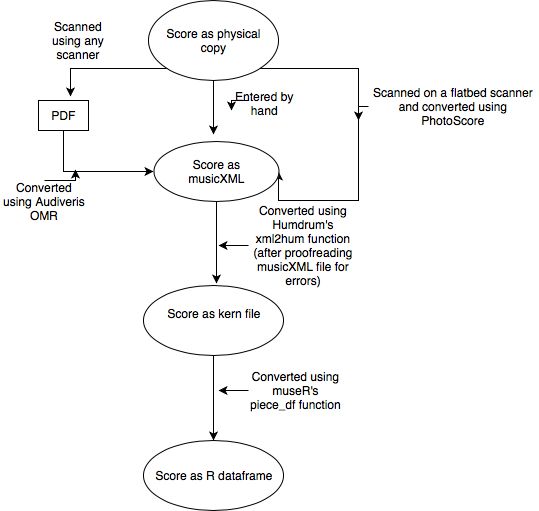
\includegraphics[scale = .5]{images/test.png}
\caption{Flowchart of the conversion process from physical score copy to dataframe in R.}
\label{subd}
\end{figure}
\section{Optical music recognition}\label{optical-music-recognition}

The vast majority of classical music scores are found solely in PDF or
physical copies. Sheet music as a form of data requires a lengthy
process of conversion before being able to be used in any analysis.
Simply scanning the scores into, say, a PDF, gives no musical semantics
and can only be viewed on screen or printed on paper. Thus, the two main
steps in reading in data from sheet music are, first, using optical
music recognition software to transform physical scores into digital
formats, and second, to read the digital format in to R where subsequent
analysis can be done.
\begin{figure}[h]
\centering
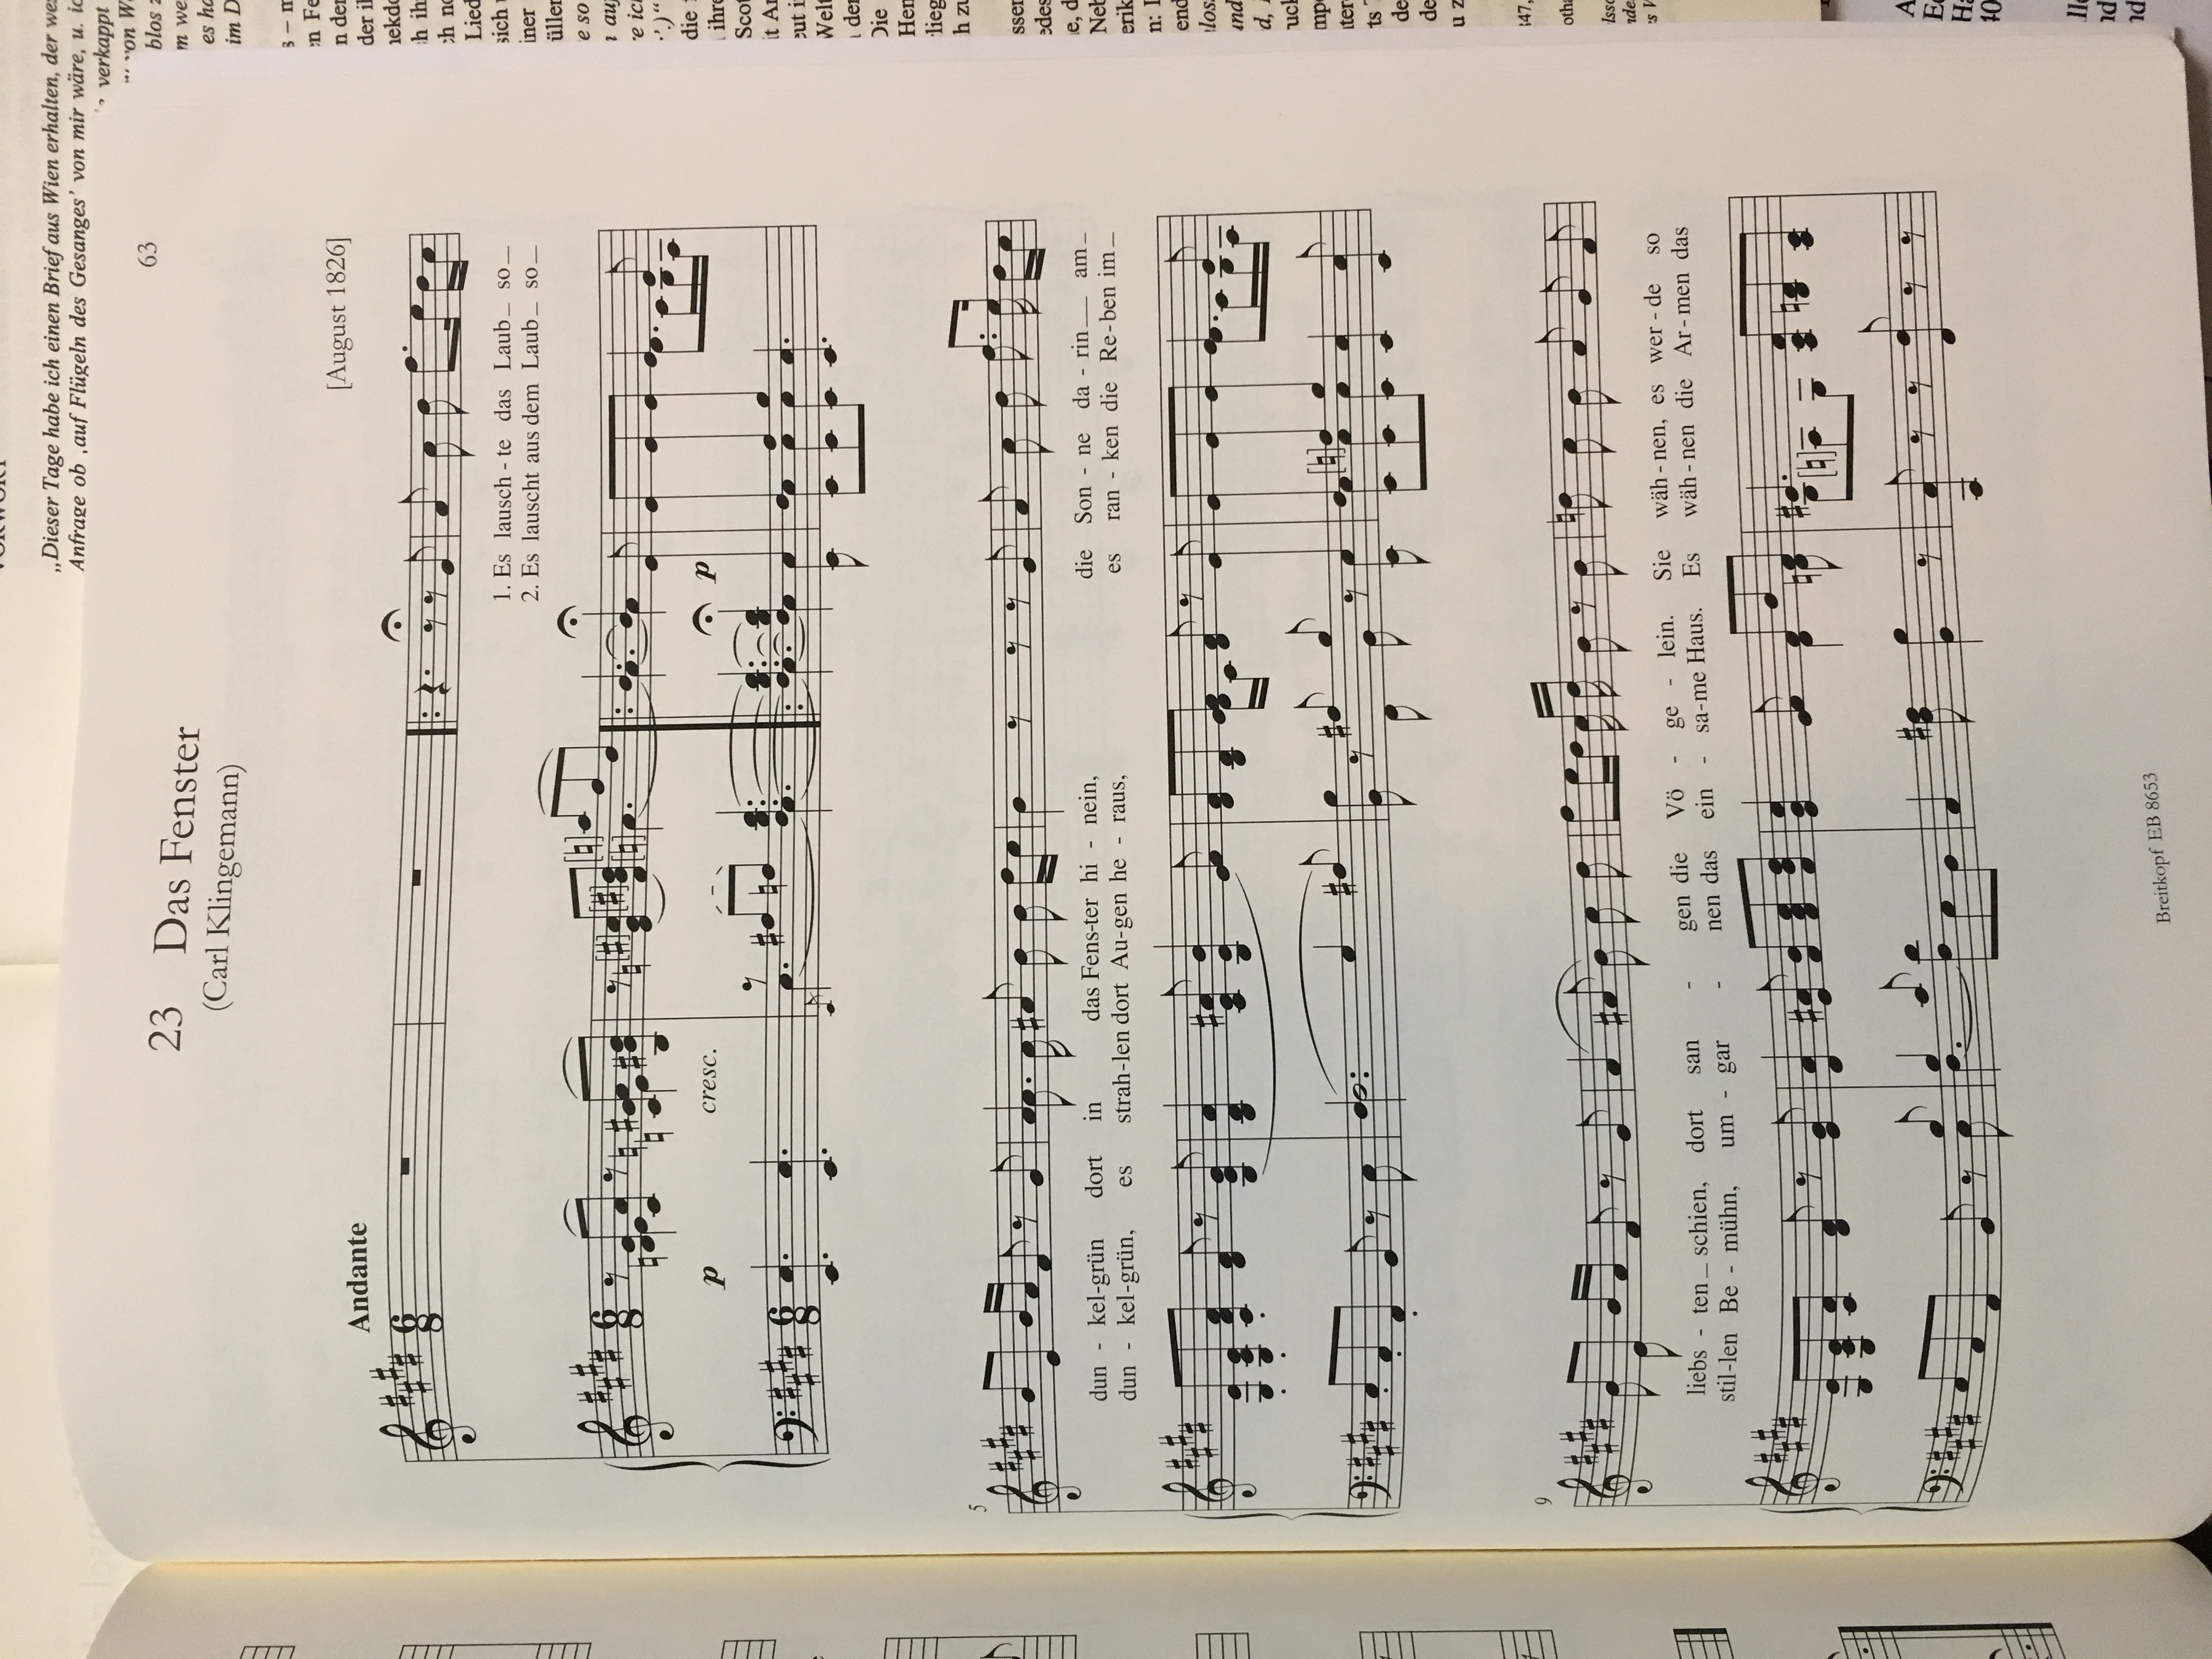
\includegraphics[scale=.50]{images/scorephoto.JPG}
\caption{Score in physical form before conversion process has started.}
\label{subd}
\end{figure}
The scores used in this paper were obtained from physical copies
available in the Reed music library. These scores were then scanned
using software designed for optical music recognition (OMR).

Optical music recognition requires learning from graphical and textual
information. The software must mainly pick up the locations of bar
lines, notes, rests, slurs, dynamic markings, tempo markings, lyrics
etc. Basic optical music recognition has been around since 1966.

Most commonly, the first step in optical music recognition is to remove
the staff lines. The staff lines are critical, as they define the basis
for the vertical definition distance of pitch, and the horizontal
distance definition of rhythm. The staff gives a normalization that is
helpful, essentially defining the size of what notes and rhythm look
like (Doermann, Tombre, \& others, 2014).

The next step is music symbol extraction and classification. These
methods include template matching, where the object in question is
compared to existing known musical symbols, simple operators, such as
analysis of bounding boxes and projections, and joining graphical
primitives, such as combining extracted objects such as notes, note
heads, and note beams to connect them in a musically correct way to form
chords. Other methods use statistical models for analyzing musical
primitives (the objects the OMR is trying to classify) such as Neural
Networks, Support Vector Machines, k-Nearest Neighbor, and Hidden Markov
Models.

The next step OMR performs is syntactical analysis and validation. This
step essentially uses defined grammars describing the organization of
music notation in terms of music symbols. This makes the classification
problem simpler, as there are existing rules and relationships between
musical symbols.

The two OMR softwares used in this paper were PhotoScore and Audiveris.
Each has its own benefits and issues. PhotoScore works by scanning the
physical score on a flatbed scanner at a high resolution. It then uses
OMR techniques to output a musicXML file that can be read in by most
music composing software, such as Sibelius, Finale or Muse Score.

Audiveris, in contrast, works by inputting a high resolution PDF and
then uses OMR techniques to output a music XML file. Often, high enough
resolution PDFs do not exist, so the physical scores must also be
scanned by any garden variety scanner.
\begin{figure}[h]
\centering
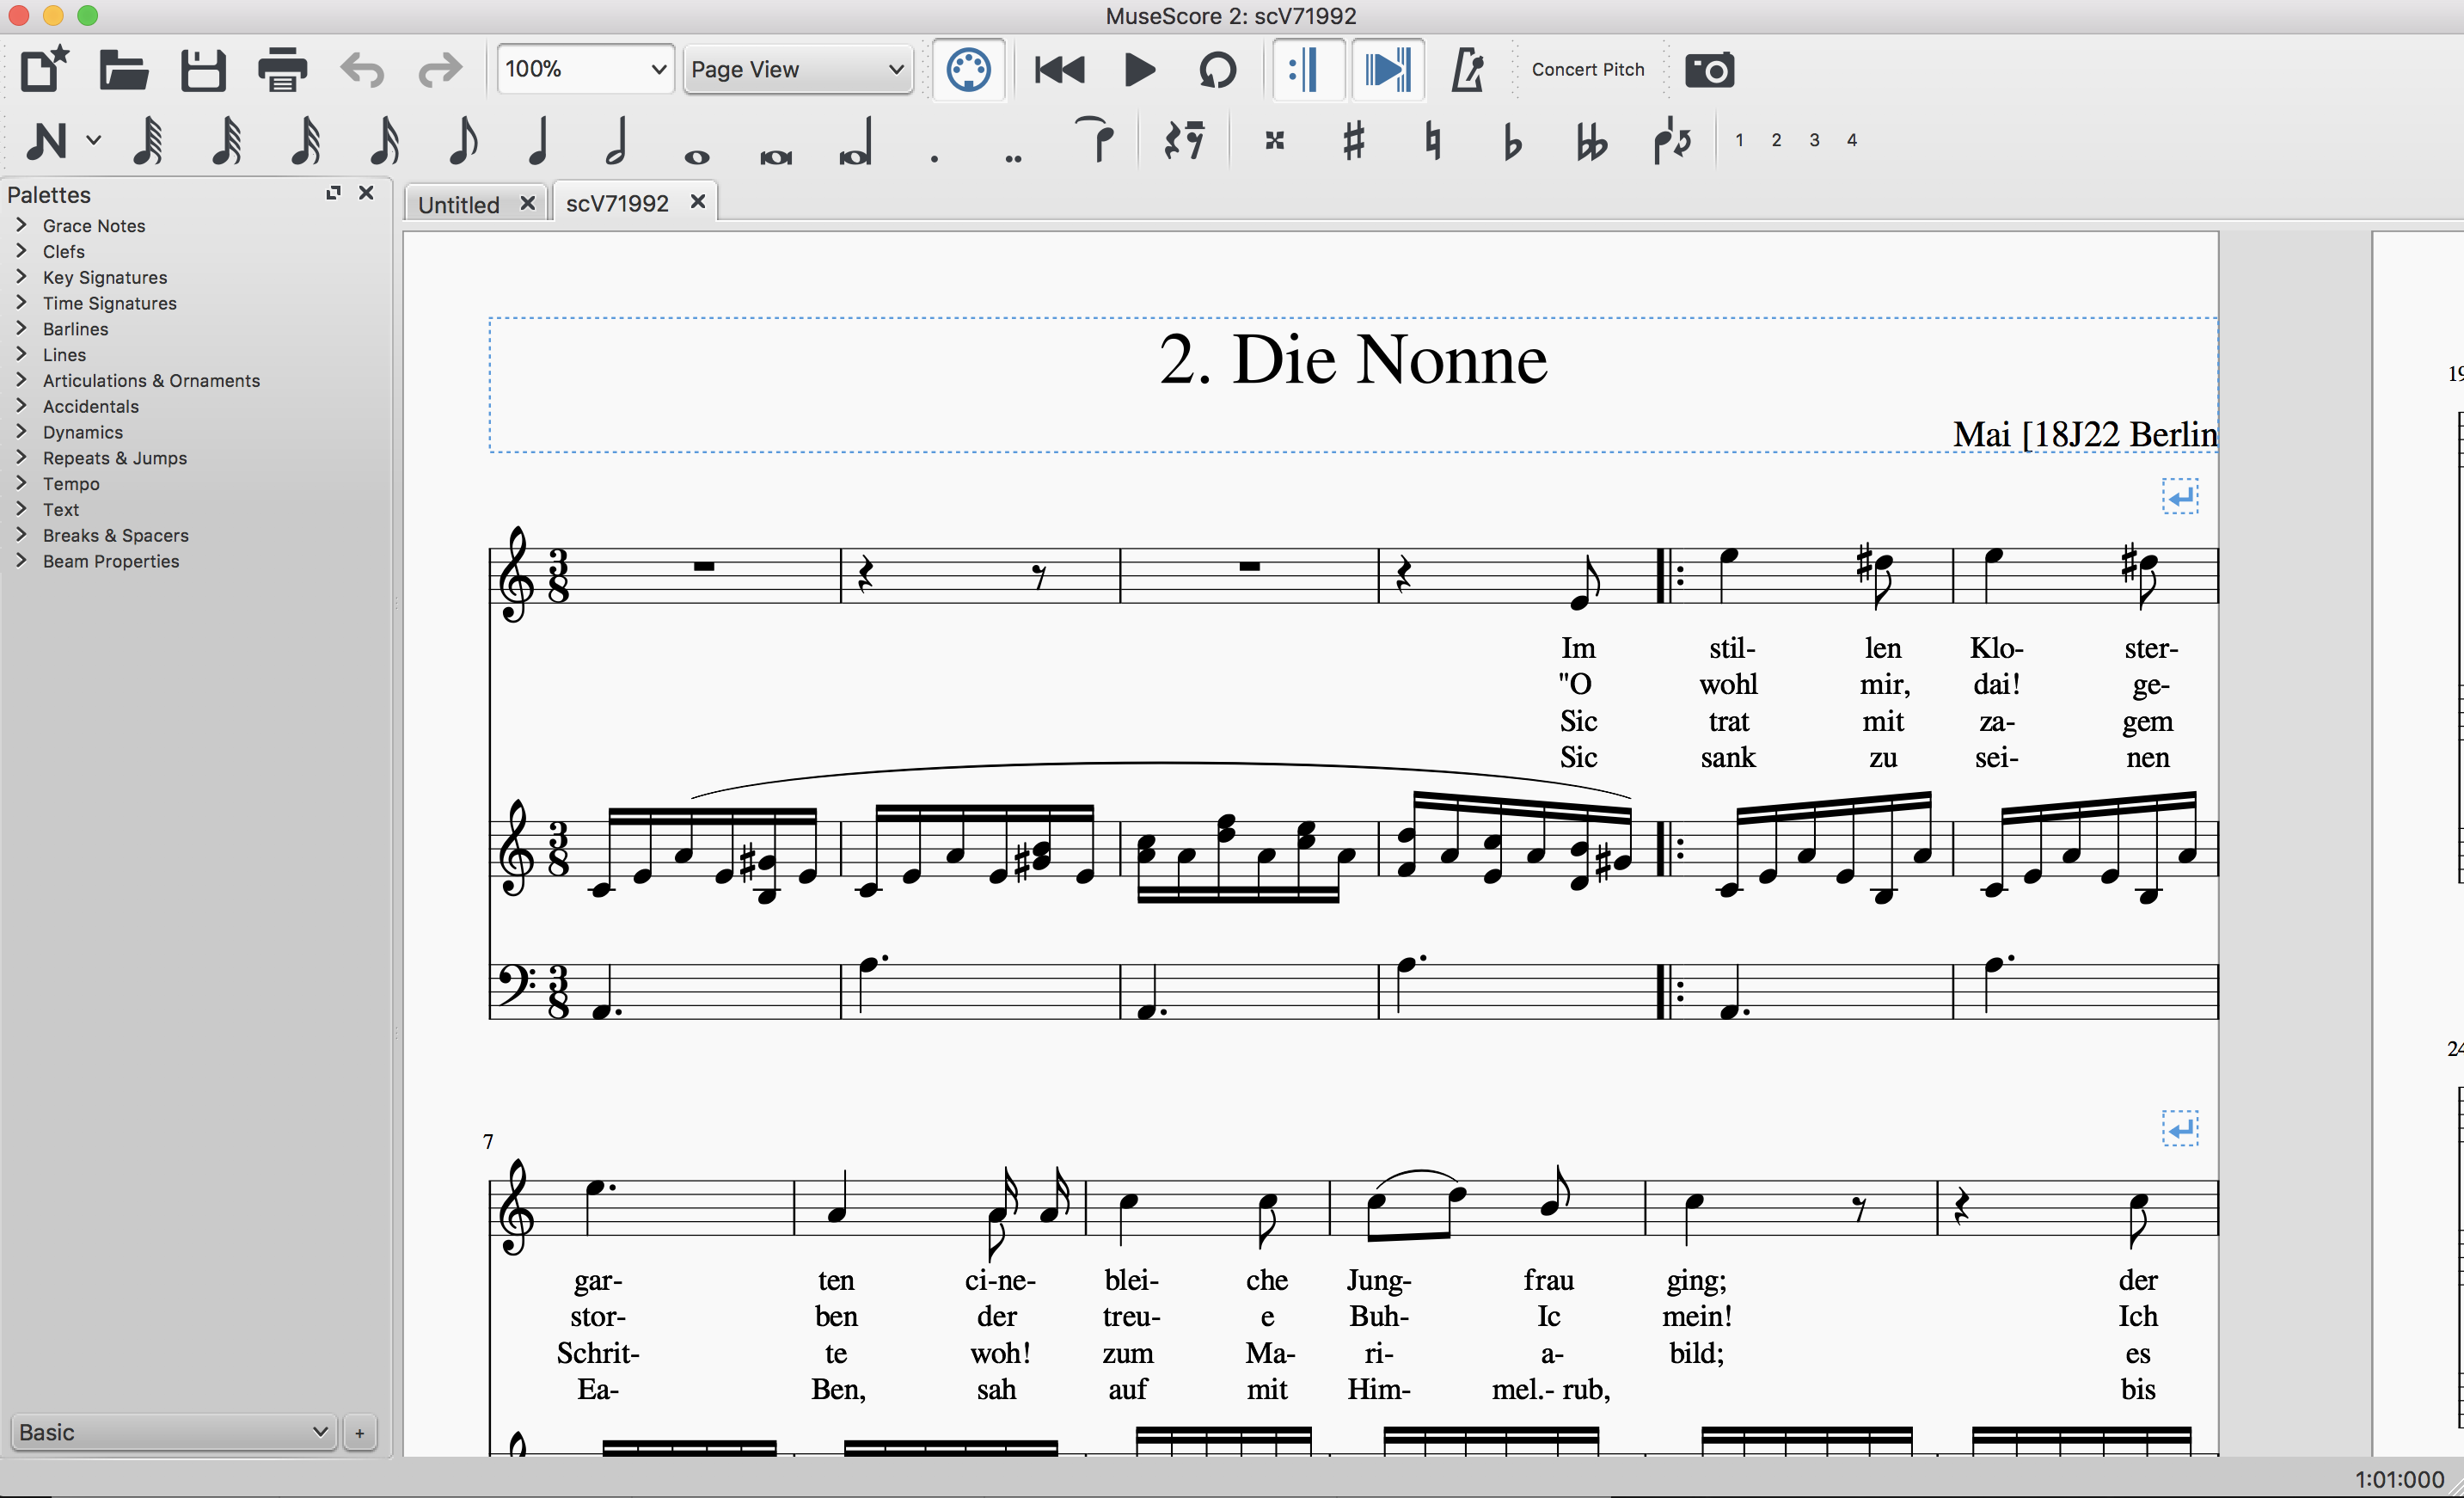
\includegraphics[scale=.30]{images/museScore.png}
\caption{A score in MuseScore format after being read by an OMR like PhotoScore or Audiveris.}
\label{subd}
\end{figure}
MusicXML is commonly used as a format for digital music, as it is
conducive to representing sheet music and music notation, and it can be
transferable to many different music software. Muse Score was chosen to
be the music software for viewing digital scores as it is a free
software that can read MusicXML.

After being scanned by PhotoScore and read into Muse Score, each piece
was proof-read and corrected. This involves looking through every piece
line by line for each bar to ``spell check'' the digital version.
PhotoScore did a good job recognizing notes, but often had issues
recognizing rhythms, and had issues keeping the structure of the piece.
Often in the scanning process clefs or bar lines were not found, causing
PhotoScore to output every staff on one line. In contrast, Audiveris
often added extra beats to measures, and assigned notes to the wrong
staff. It also always identified a bass clef as a baritone clef.

Unfortunately, the scanning process is very lengthy and time consuming,
as the scanning often gives a large number of mistakes. Often the score
must be then scanned again. In addition, the proof-reading process is
lengthy. One must check each note and rhythm for errors against the
original score, and change the incorrect notes using MuseScore. The
corrected score must then be re-outputted as a musicXML file. In
addition, there were some pieces that PhotoScore or Audiveris had a hard
time reading. These pieces were then entered into MuseScore by hand and
then proofread.

MusicXML on its own is not conducive to converting into a data frame as
representing the single half note middle C is represented in Figure 2.4.
\begin{figure}[h]
\centering
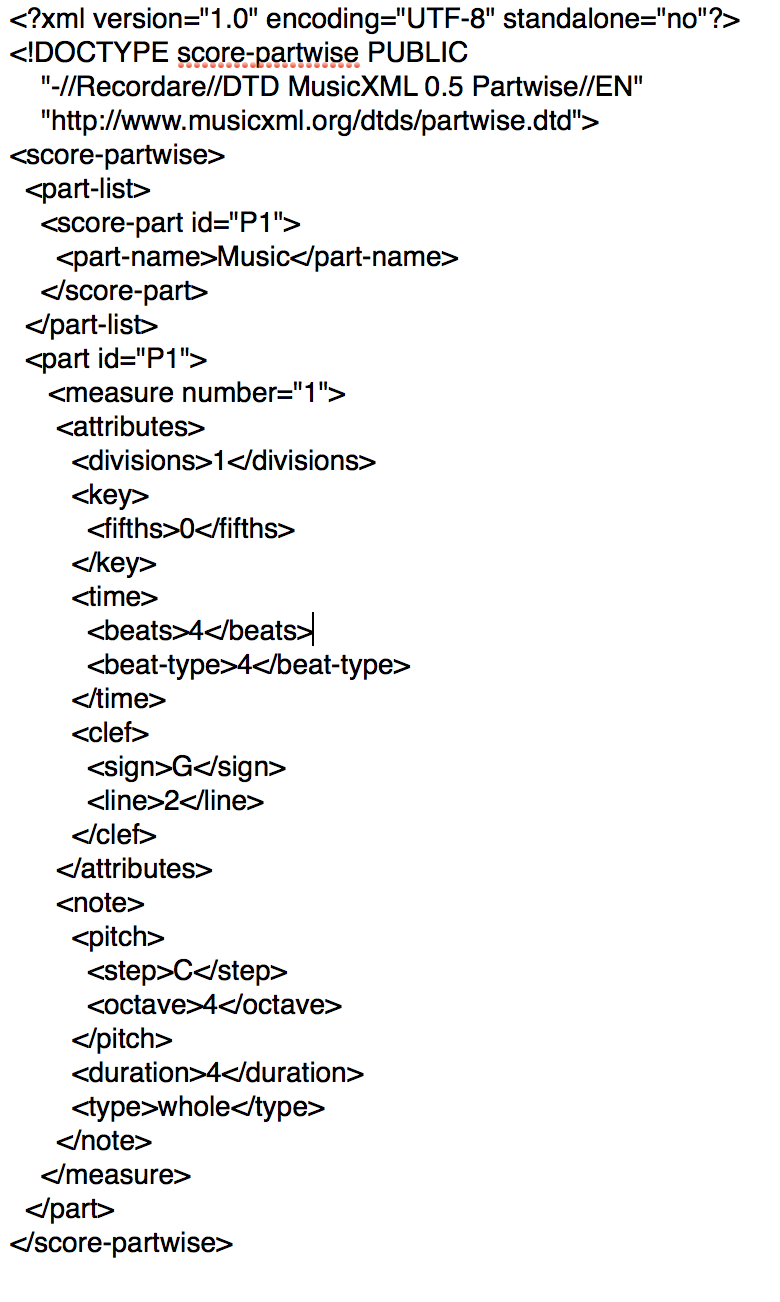
\includegraphics[scale=.4]{images/mxlc.png}
\caption{A half middle C in musicXML encoding}
\label{subd}
\end{figure}
We then need to convert into a format more easily readable into R. The
Kern Score music format is much more easily readable. It has clearly
expressed time signature, bar, beat and musical voicing information
(Mearns et al., 2010). Because of this, it is also more conducive to
being read into an R data frame. Figure 2.5 (Huron, 1994) shows how a
basic piece of music corresponds to a Kern file.
\begin{figure}[h]
\centering
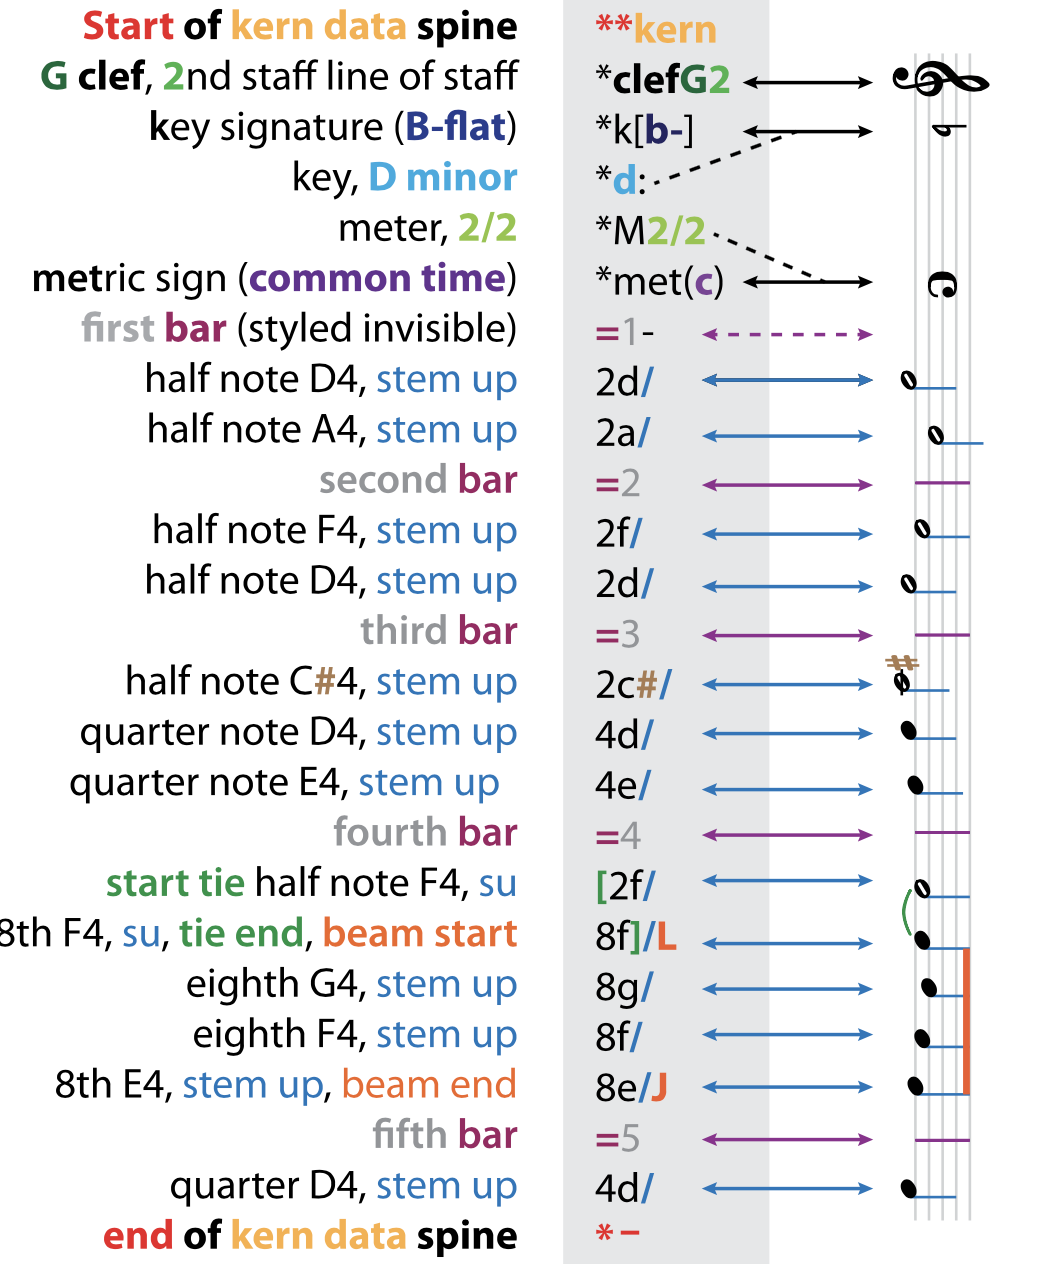
\includegraphics[scale=.50]{images/krnmusic.png}
\caption{How sheet music corresponds to kern files.}
\label{subd}
\end{figure}
Kern files are organized with columns each representing one staff of
music. Each line of a Kern file represents one note of one value of a
time base. The time base for a Kern file is based on the smallest
(shortest) rhythm value of a note found in a piece. For example, if a
piece was in 4/4 and there were sixteenth notes present there would be
16*4 rows for each measure. The ``attack'' of each note is the only note
printed, the following time while the note is held is represented with
dots in the remaining rows until a new note is sounded for that staff.
The pitch of each note is represented by the letters a through g. The
case (lower or upper) as well as the repetition (c or ccc) represents
which octave the pitch occurs. Any accidental is represented with a
\(\sharp\), -, or n symbol. Each instrument/staff in a piece is
represented using one (or more) columns called splines. For example,
most lieder consist of voice and piano. There are thus three splines,
one for voice, one for the treble clef staff of the piano, and one for
the bass clef of the piano. In addition, there are splines that contain
the text for the voice for the corresponding notes. This was not of
interest to the musical classification problem, so these splines were
removed. Chords are represented by multiple notes on the same line. For
example, if there was a half note C major triad followed by a quarter
note D flat, it would be represented as
\begin{verbatim}
2c 2e 2g
4d- . . 
\end{verbatim}
In addition, there is a lot of information about the appearance of the
piece, stem direction etc. for notes, but these factors were decided as
not important for determining style, so it was removed.

We convert to kern format by using Humdrum's function \texttt{xml2hum}
that converts a musicXML file into a kern file. Humdrum is a
computational music software used to analyze music. It is a command line
tool that has many functions for music analysis. The Kern file type can
be read much more easily into R. Compared to above, the code for a
single middle c whole note would be :
\begin{verbatim}
**kern
*clefG2
*k[c]
*M4/4
=1-
1c/
\end{verbatim}
The import\_xml\_files.sh file goes through the process of converting
scores from musicXML to .krn. Each spline needs to to be individually
converted using xml2hum. The individual splines are then converted into
the same time base (there are issues when the bass line only has half
notes and the soprano line has a lot of 32nds). This conversion
essentially adds dots as placements so that the splines can line up
correctly by measure and beat.

The CCARH has a large data base containing work mostly Baroque and
Renaissance composers already in the Kern format, which is where the
Bach data came from.

The files that were scanned (i.e.~all pieces by Felix and Fanny) need to
be separated into separate files for each staff, ie a separate file for
each instrument. In addition, since we are focused on musical style, the
text of the pieces is removed in this stage. In the case of analyzing
lieder, each piece always has two or three files. These files consist of
voice, piano right hand, and piano left hand. This is necessary to avoid
the bugs in \texttt{xml2hum} that have issues when staffs don't
necessarily match up as a result of the conversion process. This is
often caused by an inconsistency in time base.

\section{Kern to R}\label{kern-to-r}

Once we have Kern files to represent each piece we use regular
expressions to extract key information. For scanned music (Felix and
Fanny music), there are as many files are there are staffs, usually
three. MuseR's \texttt{krn2df()} and \texttt{piece\_df()} functions read
in Kern files and output a data frame in R for each piece. First the
data in Kern format are read in line by line using R's
\texttt{readLines()} function. This takes every line of the Kern file
and converts it into a vector. Each entry contains the rhythm value and
note value for all notes in that line. If there are multiple notes
played at the same time, they are all in one line. The notes are
separated by splitting up the string by spaces. This converts a single
string representing one Kern line to multiple strings each representing
one note (or dot placeholder) for one Kern line. Then each entry is
separated out into the theme and note value for each note. Each line
contains the following columns: the measure the note occurs in, the
rhythm value for the note (for example 4), note name, octave inclusive
(for example cc), note name (octave exclusive){[} C sharp{]}. In
addition, for the whole piece the key signature and meter are recorded
as columns. If there are 3 splines and each spline has at most one note
at a time, there would thus be \(3 + 3\times3=12\). If there are 3
splines and one of the splines has at most 3 values, that is equivalent
to having 5 total splines there are then \(3+3\times5 = 18\) columns.

A lot of data included in the Kern files are not necessary. For example,
we assume that whether or not a note has a stem up or stem down offers
no help in classifying composer style, so this information is removed
when converting to an R data frame.

Inspired by the Kern file type, each row of the R data frame contains
one time base value. For a given piece, the time base represents the
shortest note duration value. For example, if the shortest note a piece
contained was a sixteenth note, the time base would be 16. Each measure
then would contain 16 rows. This results in many rows of NA for certain
instruments, when a note is still being voiced, but it is not the
instance of the note being attacked.

\chapter{MuseR and features}\label{muser-and-features}

To the best of my knowledge, there is currently no package in R that has
been built to analyze sheet music. There are existing packages (such as
tuneR) that examine audio formats of music. The intention of this thesis
was to create a package, museR, that imports sheet music in the proper
form (musicXML or Kern) and does all of the analysis using R.

\section{Importing data into R}\label{importing-data-into-r}

MuseR is equipped to import data in the Kern format. The functions for
converting these files are \texttt{kern2df()} and \texttt{piece\_df()}.
These are most usefully in the form of individual splines. This allows
for naming the columns according to instrument. Figure 3.1 shows short
example piece appearing as it would look from MuseScore.
\begin{figure}[h]
\centering
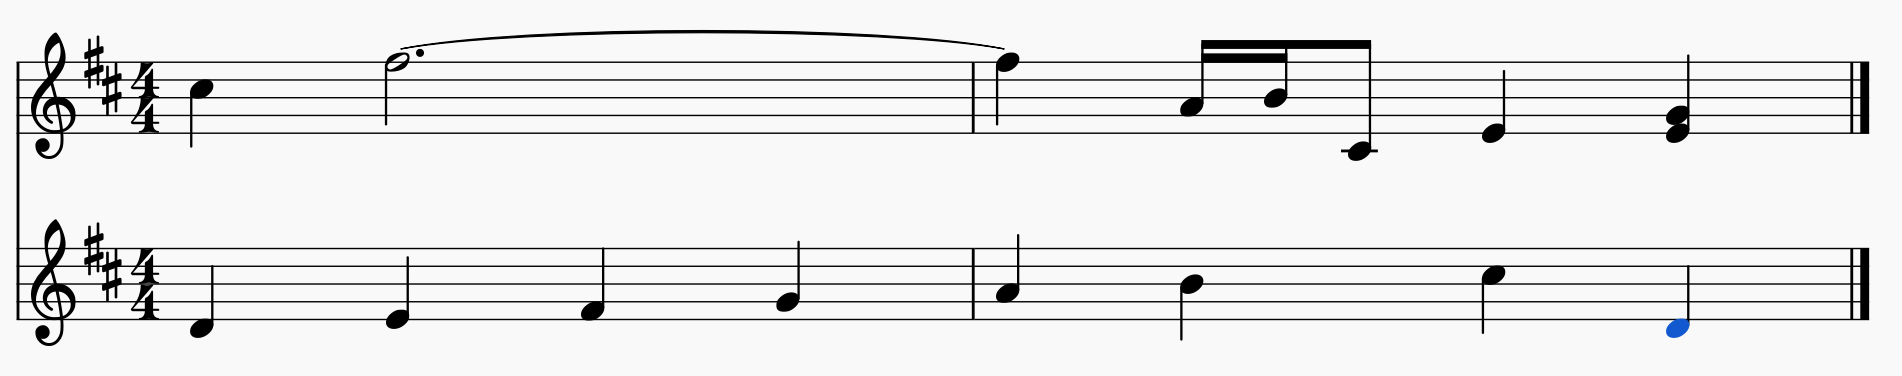
\includegraphics[scale = .5]{images/ex1m.png}
\caption{Example MuseScore format excerpt}
\label{subd}
\end{figure}
This piece would have the Kern format representation as shown in Figure
3.2.
\begin{figure}[h]
\centering
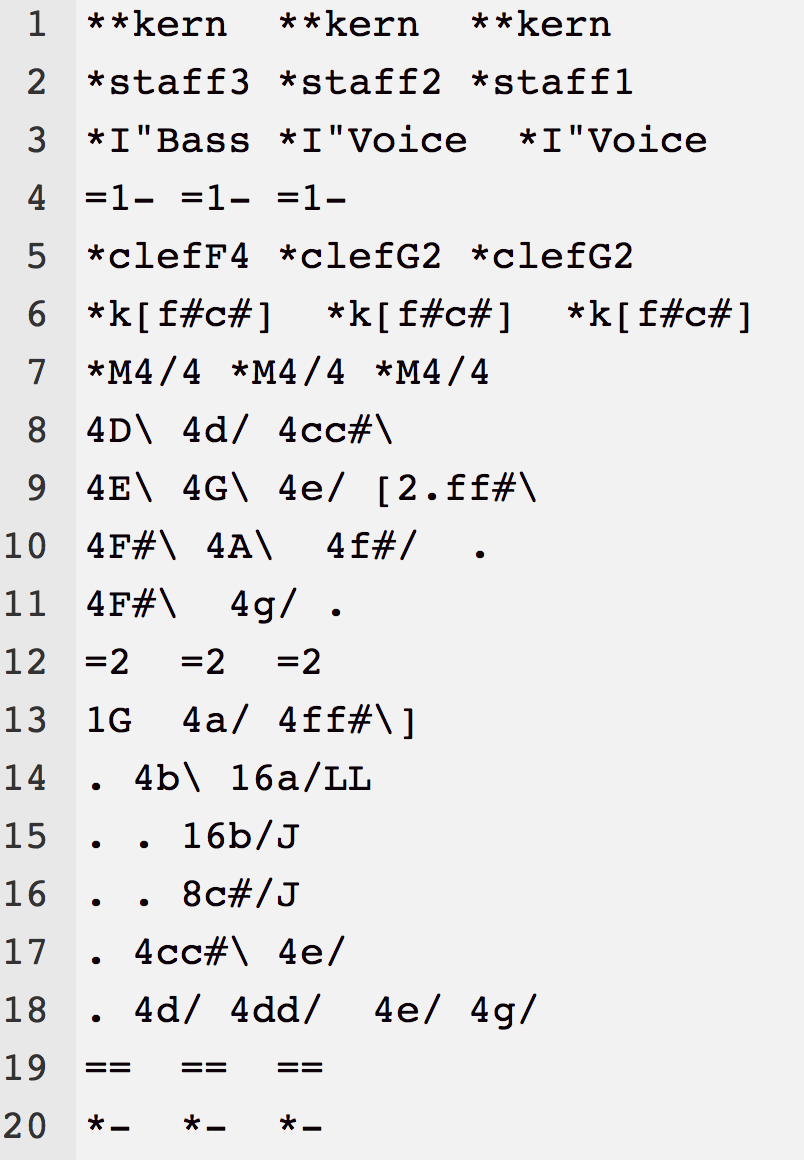
\includegraphics[scale = .5]{images/ex1k.png}
\caption{Example kern format excerpt of the above MuseScore}
\label{subd}
\end{figure}
Using museR's \texttt{piece\_df()} function to create the following data
frame.
\begin{figure}[h]
\centering
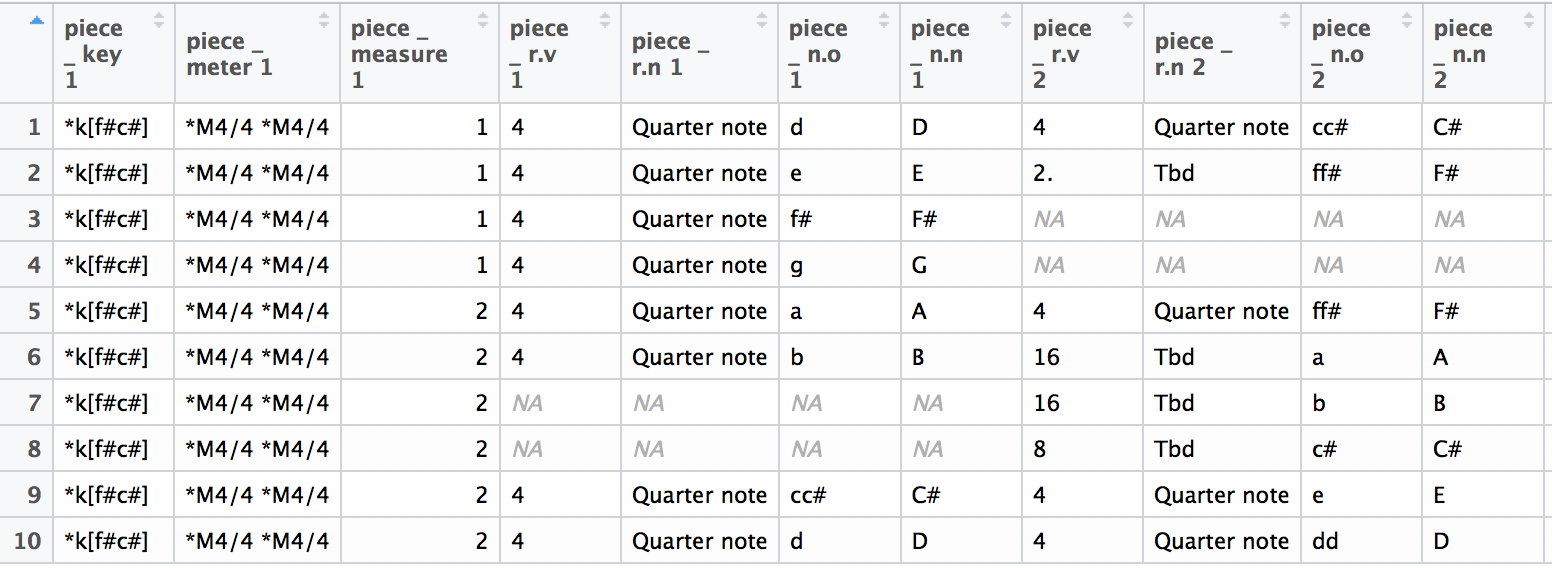
\includegraphics[scale = .5]{images/ex1r.png}
\caption{Example R data frame converted from the above MuseScore}
\label{subd}
\end{figure}
Data in R are commonly expressed as data frames. Music as a data
structure is very rugged. Expressing music as a data frame has
challenges, as music cannot be easily expressed in rectangular form.
When expressing it in rectangular form, placeholder or padding entries
must be added to account for the nonrectangularness. MuseR's
\texttt{piece\_df()} works by using regular expressions to extract note
and rhythm information. It uses NA and . values to indicate empty spaces
and duration respectively.

\section{Features currently supported in
museR}\label{features-currently-supported-in-muser}

\subsubsection{Melodic intervals}\label{melodic-intervals}

Melodic intervals, or the interval between two successive notes, are
found using the \texttt{mel\_ints()} function. It is currently only
equipped to look at melodic intervals for the top note of each staff. In
this context, it is most commonly used for analyzing melodic intervals
of the voice. The function first extracts the top line of any
instrument, and then outputs the proportion of each melodic interval
happening over the whole piece. There are 12 possible intervals that are
counted (ignoring augmented and diminished): unison, m2, M2, m3, M3, p4,
tt, p5, m6, M6, m7, M7. \texttt{mel\_ints()} outputs a vector of the
proportion of each of the intervals.
\begin{figure}[h]
\centering
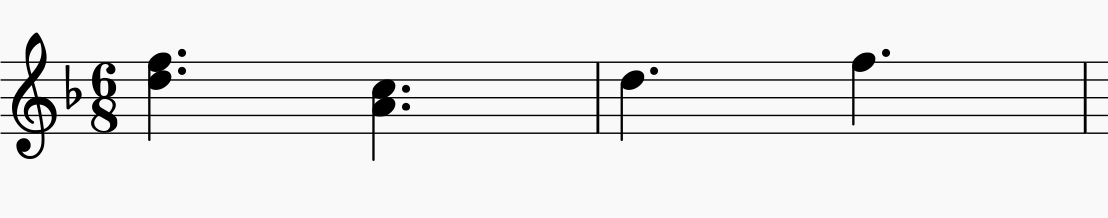
\includegraphics[scale = .5]{images/ex2.png}
\caption{Example of calculating proportion of melodic intervals}
\label{subd}
\end{figure}
For example if this function was run on the above piece, the melodic top
line intervals would be: \(\{(f,c),(c,d),(d,f)\} = \{p4,M2,m3\}\), which
would output the proportion vector \((0,1/3,1/3,0,0,1/3,0,0,0,0,0,0)\).

If we are interested in the types of melodic intervals, we can use
\texttt{consonance()} to examine the proportion of consonant (perfect,
imperfect, dissonant) intervals over the piece. This function works by
calling \texttt{mel\_ints()} and then adding up the perfect, imperfect,
and dissonant intervals proportions.

\subsubsection{Density}\label{density}

The \texttt{beat\_density()} function analyzes the average and standard
deviation of density of each measure in the piece. The function is named
``beat'' density as it only accounts for the instance a note starts. For
example if a measure consisted of a single whole note it would be only
counted once even though it is voiced the entire measure.

In the above example, the first measure would have a beat density of 4,
and the second measure would have a beat density of 2.

\subsubsection{Major\_minor}\label{major_minor}

For most musical analysis, the key of the piece is important in
determining chords, etc. The key is based on the key signature, which is
always given in a Kern file. Kern files from CCARH have the key of the
piece given, but scanned files do not. For kern files from CCARH,
\texttt{Major\_minor()} extracts the key given by the Kern file. for
scanned files, \texttt{Major\_minor()} identifies the two options for
key given the key signature. For example, if there was a key signature
with one sharp, the options would be G Major or E minor. The tonic for
each option is identified, and then the count of instances of both
choices for tonic is made. The key is determined by which of the options
for tonic has the higher count.

\subsubsection{Scale degree frequencies}\label{scale-degree-frequencies}

Once the key of a piece is determined, the proportion of each scale
degree is calculated. The scale degrees consist of: Tonic, Supertonic,
Mediant, Submediant, Dominant, Submediant, and Leading tone. In the
example above, if we assume the key is F major, the tonic has a tonic
scale degree proportion of 2/6, the mediant 1/6, dominant, 1/6,
submediant, 2/6.

\subsubsection{Frequency of rhythm use}\label{frequency-of-rhythm-use}

We determine the frequency using \texttt{rhythm\_freq()} to find the
most common types of rhythm: half notes, dotted half notes, quarter
notes, dotted quarter notes, eighth notes, dotted eight notes, sixteenth
notes, and thirty second notes.

\subsubsection{Length}\label{length}

We use \texttt{length\_measures()} as a feature for the length of a
piece. It is calculated by finding how many measures the piece has.

\chapter{About Classification Models}\label{about-classification-models}

Classification problems attempt to divide observations (features) into
groups (composer) based on similarities in the observations. A
classifier is some function \(f\) that maps a vector of input features
\(x \in X\) to a composer \(y \in Y\) or possibly a probability of a
composer \(P(Y = y) \in [0,1]\). The notation used in this chapter is
inspired by \emph{The Elements of Statistical Learning} (Friedman,
Hastie, \& Tibshirani, 2001) and \emph{An Introduction to Statistical
Learning} (James, Witten, Hastie, \& Tibshirani, 2013).

Our features space \(X\) is an \(n \times p\) matrix, where \(n\) is the
size of our data, and \(p\) is the number of predictors. Each \(X_i\) is
vector of values for a certain feature. \(x_{ij}\) denotes the
\(i^{th}\) values of the \(j^{th}\) feature. This \(X\) contains the
information of the extracted features that hopefully will be useful in
determining the composer of the piece. If the features are different
enough between the composers, i.e., that the features encode some
difference of unconscious (or conscious) style, we can then build and
fit models that leverage this difference. These models can both explain
the relationship and difference of the features between composers, and
use the way the fitted model explains the differences to predict the
composer of a piece if we know the same features for that piece.

In addition to the features for each piece, each piece has a composer
(response), known or unknown, that we denote by \(Y\). The \(i^{th}\)
piece has composer \(Y_i\) where \(i \in 1, \ldots, n\) In our case we
have \(Y \in \{\text{Fanny},\text{Felix}, \text{Bach}\}\), or more
generally, \(y \in \{\text{list of composers}\}\). Since the options for
composer are in a discrete set, we can divide the input features space
into different groups, or regions, that are labeled according to the
classification of composer a model assigns or predicts.

\section{Supervised Methods}\label{supervised-methods}

Supervised methods involve learning about data with knowledge of the
response or composer. Classification models rely on supervised
techniques to predict composers. These models are built using the
observations with their associated response.

\subsection{Logistic Regression}\label{logistic-regression}

Knowing the conditional probability \(P(Y = k|X)\), or the probability
that a piece has a certain composer, given the features of that piece,
results in an optimal classification. Logistic regression directly
models \(P(Y = k|X)\) by using the logistic function. The idea is to
model the posterior probabilities of each of the \(K\) classes as linear
functions in \(x\) and requiring that the probabilities sum to 1. As is
often the case, we use logistic regression to model a binary response:
where there are two options for composer. Thus in the case of a binary
response we can use an indicator function with coding 0/1. We then name
\(p(X) = P(Y=1|X)\) The model has the form:
\[ \log \bigg( \frac{p(X)}{1-p(X)} \bigg) = \beta_0 + \beta_1 X_1 + \cdots + \beta_pX_p\]

where which can be written as:

\[ p(X) = \frac{e^{\beta_0 + \beta_1X_1 + \cdots + \beta_pX_p}}{1 +e^{\beta_0 + \beta_1X_1 + \cdots + \beta_pX_p} }\]

We estimate the regression coefficients, \(\beta_i\), by using maximum
likelihood. This results in coefficient estimates such that for the
predicted probability \(\hat{p}(x_i)\) for the composer of each piece
corresponds as closely as possible to the observed composer. The
log-likelihood for \(N\) observations is:

\[ \ell(\beta) = \sum_{i = 1}^N \big\{y_i\log p(x_i;\beta) + (1-y_i)\log(1-p(x_i;\beta))\big\} = \sum_{i = 1}^N \big\{y_i\beta^Tx_i - \log(1 + e^{\beta^Tx_i})\big\}\]
We then choose \(\beta\) to maximize \(\ell(\beta)\).

\subsubsection{Lasso model selection}\label{lasso-model-selection}

The Lasso penalty is a shrinkage method proposed by Robert Tibshirani in
1996. Lasso regression works by giving a penalty to the magnitude of
regression coefficients. The intercept is not included in the penalty.
It can be somewhat equivalent to performing variable selection, as for
high enough penalties (or \(\lambda\)), coefficients shrink to zero. It
is often used in linear regression, but can be expended to logistic
regression and other generalized linear models. For logistic regression,
the lasso works by choosing coefficients \(\beta_\lambda^L\) that
minimize

\[ \ell(\beta) + \lambda \sum_{j = 1}^p |\beta_j| \]

where \(\ell(\beta)\) is the log-likelihood function for logistic
regression. This is equivalent to maximizing \(\ell(\beta)\) subject to
\(\sum_{j=1}^p|\beta_j| < s\) (Tibshirani, 1996).

\subsection{Linear Discriminant
Analysis}\label{linear-discriminant-analysis}

Whereas logistic regression involves directly modeling
\(P(Y = k | X =x)\), linear discriminant analysis (LDA), estimates these
values less directly by using Bayes Theorem. When classes are well
separated or if \(n\) is small and the distribution of predictors is
approximately normal, logistic regression estimates can be unstable,
which is not the case for LDA. LDA is also popular when there are more
than two response cases.

To perform LDA we must first model the distribution of each of the
features that make up \(X\) in each of the response classes,
\(P(X = x|Y)\). We denote \(f_k(X) = P(X = x| Y = k)\) as the
class-conditional density of \(X\) in class \(Y = k\). We denote the
prior for class \(k\), \(\pi_k\), or the probability that a chosen
observation is from the \(k^{th}\) class. We have that
\(\sum_{k=1}^K \pi_k = 1\). Using Bayes' theorem to calculate
\(P(Y = k |X)\) gives us the following:

\[ P(Y = k | X = x) = \frac{f_k(x)\pi_k}{\sum_{l = 1}^Kf_l(x)\pi_l}\]

We thus must have a model to find \(f_k(x)\). Different discriminant
analysis techniques do this different ways. LDA assumes a multivariate
Gaussian density, given by:
\[f_k(x) = \frac{1}{(2\pi)^{p/2}|\mathbf{\Sigma}_k|^{1/2}}e^{-\frac{1}{2}(x-\mu_k)^T\mathbf{\Sigma}_k^{-1}(x - \mu_k)},\]
where \(\mu_k\) is the mean parameter for the \(k\)th class and
\(\Sigma_k\) is the covariance matrix for the \(k\)th class.

In addition, LDA assumes that the covariance matrix is equal for every
\(k\): \(\mathbf{\Sigma}_k = \mathbf{\Sigma}\) \(\forall\) \(k\). Other
discriminant models do not make this assumption. We also assume
\(\hat{\pi}_k = N_k/N\) where \(N_k\) is the number of class - \(k\)
observations,

Using the formula for \(P(Y = k|X=x)\) as stated above, we can use LDA's
assumption of \(f_k(X = x)\) which results in the discriminant function:

\[ \delta_k(x) = x^T\mathbf{\Sigma}^{-1}\mu_k - \frac{1}{2}\mu_k^T\mathbf{\Sigma}^{-1}\mu_k + \log \pi_k \]

These functions are known as \(\textit{linear discriminant functions}\).
We predict the class by finding the maximum value of the discriminant
functions of all \(k\).

\subsection{Naive Bayes}\label{naive-bayes}

The Naive Bayes classifier is often used for musical classification as
it is good when the dimension \(p\) of the features space is large. Like
LDA, it also involves modeling \(P(Y = y | X =x)\) by using assumptions
of the form of \(f_i(X)\) and using Bayes Theorem. Naive Bayes makes the
(naive) assumption that all the features are independent for a given
class \(i\), \[f_i(X) = \prod_{k = 1}^p f_{ik}(X_k).\] These marginals
are often estimated by using a Gaussian distribution, ie that
\(f_{ik}(X_k) = \frac{1}{\sqrt{2\pi\sigma_k^2}}e^{\frac{(x - \mu_k)^2}{2\sigma_k^2}}\).
In practice, the independence assumption is not the case, but the model
still performs surprisingly well.

\subsection{\texorpdfstring{\(k\)-nearest
neighbor}{k-nearest neighbor}}\label{k-nearest-neighbor}

Another method for classification is \(k\)-nearest neighbor methods. It
uses observations from a training set of the data. Then for a new
observation in a testing set at point \(x_0 = x_1 \ldots x_p\), it finds
the \(k\) closest points in the training set, and classifies \(x_0\) as
the majority vote of the responses for the \(K\) neighbors. Euclidean
distance is often used as the metric for closeness, although other
methods exist. Euclidean distance is defined as \(d = |x_{(i)} - x_0|\).
After the \(K\) nearest neighbors are found, the predicted class for
\(x_0\) is assigned to be the mode of the classes of the neighbors.

\subsection{Random Forests}\label{random-forests}

Tree-based methods are another form of classifier. Tree based methods
involve segmenting the predictor space into smaller regions that are
similar in their response. To classify a point \(x_0\), we take the mode
of the classes of training set observations in the smaller region where
\(x_0\) lies, and assign the class of \(x_0\) as the mode. To create the
tree, we recursively split the predictor space into two smaller regions,
where the split point is known as a node. Nodes with high node purity
are choices where the two resulting regions have mostly the same class
in the region. We chose a good split based on the split with highest
node purity. The Gini index is often used to measure node purity,
defined as \(G = \sum_{k = 1}^K \hat{p}_{mk}(1 - \hat{p}_{mk})\), where
\(\hat{p}_{mk}\) is the proportion of observations in the \(m\)th region
of the \(k\)th class. If the Gini index is small, this indicates that a
region contains mostly observations from a single class.

Random forests offer an improvement over trees in general. They create a
``forest'' of decision trees on bootstrapped training samples. In each
of the trees in the forest, a random sample of \(m\) predictors are
chosen to create the tree. For random forests, \(m = \sqrt{p}\)
typically. Because strong predictors are often chosen for the first
split of the tree, choosing only a random sample of the predictors to
build the tree makes the trees in a random forest significantly
different from each other. This choice helps in decorrelating the trees.
To predict the class of a piece, we then take the majority vote of the
class predicted for each tree in the random forest.

\section{Unsupervised methods}\label{unsupervised-methods}

Unsupervised methods are methods where the response is not used. The
methods involve learning structures in the data without any labeled
response or composer. Some unsupervised methods, such as PCA, can be
used for later models that rely on supervised methods.

\subsection{Principal component analysis
(PCA)}\label{principal-component-analysis-pca}

Principal component analysis (PCA) transforms the features space into a
lower dimensional representation. It chooses the transformed features to
have maximal variance and be mutually uncorrelated.

Principal component analysis can be useful when the predictors are
correlated. We suspect many of our features are correlated, due to
certain patterns in music, as well as the way we created our features.
These relationships are caused by similarity in the features, and from
music theory rules. For example, if there is a high frequency of first
scale degrees, we might expect a high frequency of chords that include
the first scale degree. Another example, if we had a high frequency of
seventh scale degrees, we would expect them to resolve to the first
scale degree.

Principal component analysis is also helpful when there are many
predictors, and we want to deal with a smaller dimension of predictor
space. To do this, we choose to use fewer principal components than
features, and as principal components are chosen in a way to maximize
the variability in the data, so including fewer principal components
than features still ideally gives a good representation of the initial
data. Used in supervised methods, the transformed features from PCA can
be used to fit models instead of the original features.

As an unsupervised method, PCA can inform about latent meta variables.
Meta variables are features included in the data that aren't
specifically measured by individual features. PCA explores these by
giving similar weights to features that are correlated with each other.
Thus original features that have similar PCA scores have similar
interpretability.

Principal components transforms the feature space. If our original
features are \(X_1,X_2,\ldots,X_p\), we transform the features to
\(Z_1,Z_2,\ldots,Z_M\), where \(M \leq p\). Each \(Z_i\) is a linear
combination of the original predictors, ie,
\(Z_m = \sum_{j = 1}^p \phi_{jm}X_j\), for constants
\(\phi_{1m},\phi_{2m},\ldots,\phi_{pm}\) for \(m = 1,\ldots,M\). Given
an \(n\times p\) data set \(\mathbf{X}\) where \(x_{ij}\) is the
\(i^{th}\) instance of the \(j^{th}\) feature, we solve for the
\(m^{th}\) principal component loading vector
\(\phi_m = \phi_{1m},\phi_{2m},\ldots,\phi_{pm}\) that solves the
optimization problem:
\[\max_{\phi_{1m},\ldots,\phi_{pm}} \bigg\{\frac{1}{n}\sum_{i=1}^n\bigg(\sum_{j=1}^p \phi_{jm}x_{ij}\bigg)^2\bigg\},\]
where the \(\phi\)s are subject to \(\sum_{j = 1}^p\phi_{jm}^2 = 1\).
Our principal components are then calculated as
\(z_{im} = \sum_{j = 1}^p\phi_{jm}x_{ij}\).

The loadings of the first principal component, \(\phi_1\) thus determine
the direction in the feature space with the most variance, \(Z_1\), or
the scores of the first principal component is then a new feature in our
transformed feature space. We continue calculating \(Z_i\), where each
following \(Z_i\) has the maximal variance in a direction uncorrelated
to the previous principal components.

Before PCA is performed, we center and scale all features to have mean
zero and standard deviation one, as initially the scale of some features
are not the same. This would lead to issues in the loadings, as the
features with higher scales would automatically have the higher
variance.

We can observe the proportion of variance explained by each principal
component. This is usually visualized in a skree plot. The number of the
principal component is plotted on the x-axis, and the percentage of
variance which that principal component accounts for is on the y-axis.
We can use this information to decide how many principal components to
use. We often choose the cut-off principal component at an ``elbow'', or
where the decrease in variance explained by an additional principal
component starts to decrease.

\subsection{K-means}\label{k-means}

\(K\)-means is a form of unsupervised learning where we only use the
features without the associated class of composer. When given a \(K\) or
number of clusters, the algorithm assigns each piece to a cluster. This
is used to see if there are any latent groupings in the feature space.
If composers are differentiable by their features, we might expect that
\(K\) means would differentiate the clusters similar to the difference
in composer. K-means clustering minimizing the within-cluster variation
\(W(C_k)\) for each cluster \(C_k\). Often we define the within-cluster
variation by squared Euclidean distance, so
\[W(C_k) = \frac{1}{|C_k|} \sum_{i,i' \in C_k}\sum_{j = 1}^p (x_{ij} - x_{i'j})^2 \]
where \(|C_k|\) is the number of observations in the \(k\)th cluster.

\chapter{Exploratory Data Analysis}\label{exploratory-data-analysis}

Before fitting any classifiers, we first want to perform exploratory
data analysis to examine visually any patterns or separations between
variables and composer. This is done by looking at individual density
plots of each variable for each composer, looking at correlation
structures in the features, and using PCA as an unsupervised method to
gain insight into the feature space. We examine two cases, features for
Bach/not Bach, where not Bach is the pieces of Fanny Hensel and Felix
Mendelssohn combined. We denote this as Bach/Mendelssohn. We also
examine the features for Fanny/Felix.

\section{Key for feature
abbreviations}\label{key-for-feature-abbreviations}
\begin{longtable}[]{@{}ll@{}}
\caption{Abbreviations for features and corresponding meanings. The
features of Fanny and Felix are the same but begin with
f.}\tabularnewline
\toprule
\begin{minipage}[b]{0.11\columnwidth}\raggedright\strut
name\strut
\end{minipage} & \begin{minipage}[b]{0.83\columnwidth}\raggedright\strut
meaning\strut
\end{minipage}\tabularnewline
\midrule
\endfirsthead
\toprule
\begin{minipage}[b]{0.11\columnwidth}\raggedright\strut
name\strut
\end{minipage} & \begin{minipage}[b]{0.83\columnwidth}\raggedright\strut
meaning\strut
\end{minipage}\tabularnewline
\midrule
\endhead
\begin{minipage}[t]{0.11\columnwidth}\raggedright\strut
dens\_.\strut
\end{minipage} & \begin{minipage}[t]{0.83\columnwidth}\raggedright\strut
Density of notes: mean and standard deviation\strut
\end{minipage}\tabularnewline
\begin{minipage}[t]{0.11\columnwidth}\raggedright\strut
cons\_.\strut
\end{minipage} & \begin{minipage}[t]{0.83\columnwidth}\raggedright\strut
Type of melodic intervals: imp(imperfect), dis(dissonant),
perf(perfect)\strut
\end{minipage}\tabularnewline
\begin{minipage}[t]{0.11\columnwidth}\raggedright\strut
rf.\strut
\end{minipage} & \begin{minipage}[t]{0.83\columnwidth}\raggedright\strut
Rhythm frequency: 2(half), 2d(dotted half), 4 (quarter), 4d(dotted
quarter), 8(eighth), 8d(dotted eighth), 16(sixteenth) ,32(thirty
second)\strut
\end{minipage}\tabularnewline
\begin{minipage}[t]{0.11\columnwidth}\raggedright\strut
sf\_.\strut
\end{minipage} & \begin{minipage}[t]{0.83\columnwidth}\raggedright\strut
Scale degree frequency: 1 to 8\strut
\end{minipage}\tabularnewline
\begin{minipage}[t]{0.11\columnwidth}\raggedright\strut
len\strut
\end{minipage} & \begin{minipage}[t]{0.83\columnwidth}\raggedright\strut
Length of the piece\strut
\end{minipage}\tabularnewline
\bottomrule
\end{longtable}
\section{Bach and Mendelssohns}\label{bach-and-mendelssohns}

Figure 5.1 shows density plots for each of the predictors used. We can
see some difference of that feature being used by composer in the
density features, and some of the rhythmic frequency features,
especially use of eighth notes and sixteenth notes. The peaks for Bach
are mostly narrower than those for Mendelssohn. One can suspect the
difference in density is partially caused by the type of piece of Bach
and Mendelssohn. We might expect that solo pieces, such as those in the
Bach data set would have lower densities then for lieder, as in the
Mendelssohn data set, which also include voice.
\begin{figure}[H]
\centering
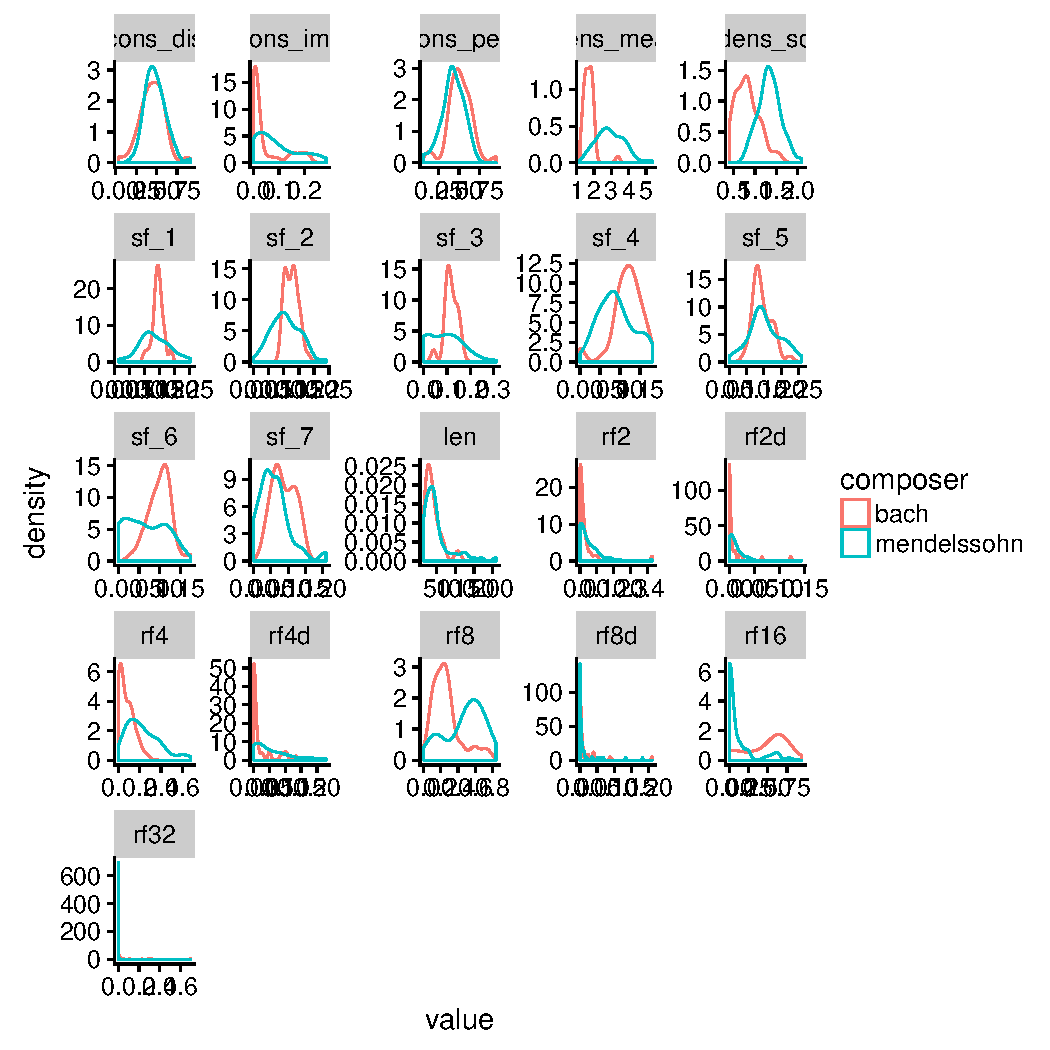
\includegraphics[scale = .7]{images/distribution_b.pdf}
\caption{Density plot for each feature of Bach/Mendelssohn. Red represents Bach and blue represents the Mendelssohns.}
\label{subd}
\end{figure}
\begin{figure}[H]
\centering
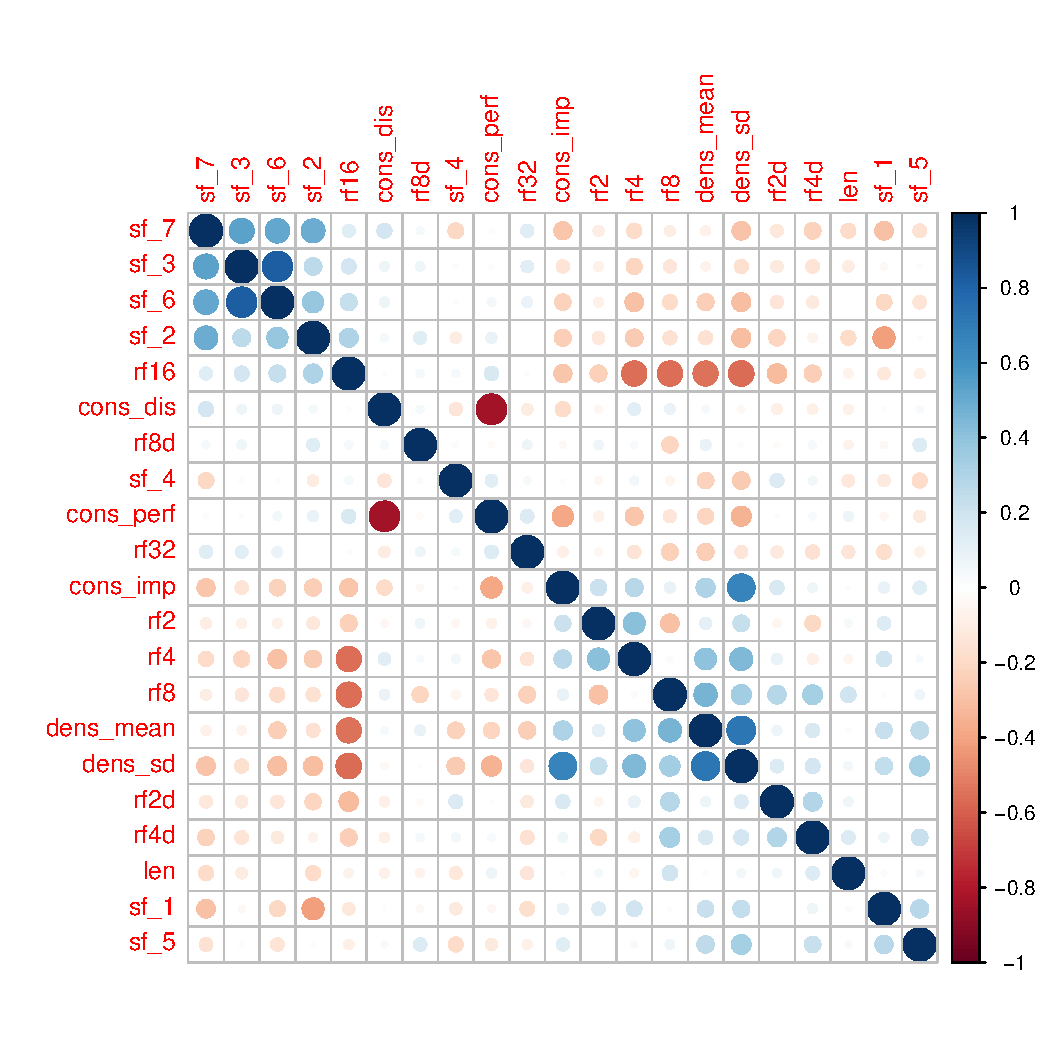
\includegraphics[scale = .7]{images/cor_circles_b.pdf}
\caption{Correlations between features of Bach/Mendelssohn.}
\label{subd}
\end{figure}
Figures 5.2 is a visualization of the correlation matrix. The size of
the circle represents the absolute value of correlation between the two
predictors. We can see higher correlations between perfect consonances
and dissonant consonances. This is to be expected, as a higher frequency
of perfect consonances necessarily means a lower frequency of dissonant
consonances. We also see high negative correlations between frequency of
sixteenth notes and density, and frequency of eight notes. In addition
we see high positive correlations between frequency of second, third,
sixth, and seventh scale degree. It is likely that these negative
correlations are due to structures in music theory or sensible melodic
compositional technique.
\begin{figure}[H]
\centering
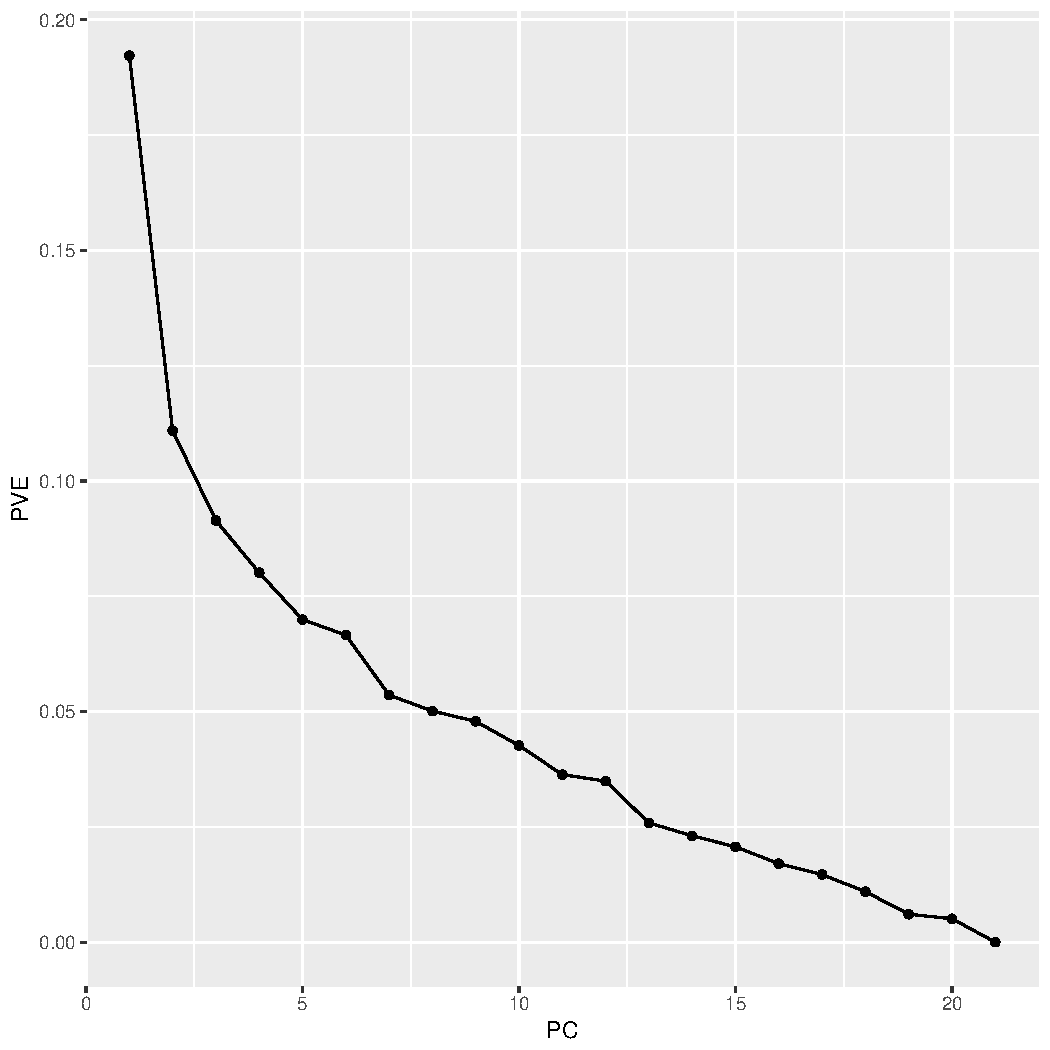
\includegraphics[scale = .7]{images/skree_b.pdf}
\caption{Skree plot of the PCA's.}
\label{subd}
\end{figure}
Figure 5.3 shows the skree plot of the principal components of Bach and
Mendelssohn. For each principal component used (shown on the x-axis), we
have the corresponding percentage of variance explained (y-axis). Often
when using PCA for dimension reduction, we often look for an elbow in
the skree plot. This is done to choose the smallest number of principal
components needed to explain a sizable amount of the variation in the
feature space. There is a possible elbow at the second principal
component. This indicates that we might be able to perform analysis
using only the first two principal components. However, especially
considering that our data are not very separable, we likely would likely
want to use more information in our model. As a similar result occurred
for Brinkman, in our analysis we will use the principal components that
account for 85\% of the variance. In the Bach/Mendelssohn case this
corresponds to using 11 principal components.
\begin{figure}[H]
\centering
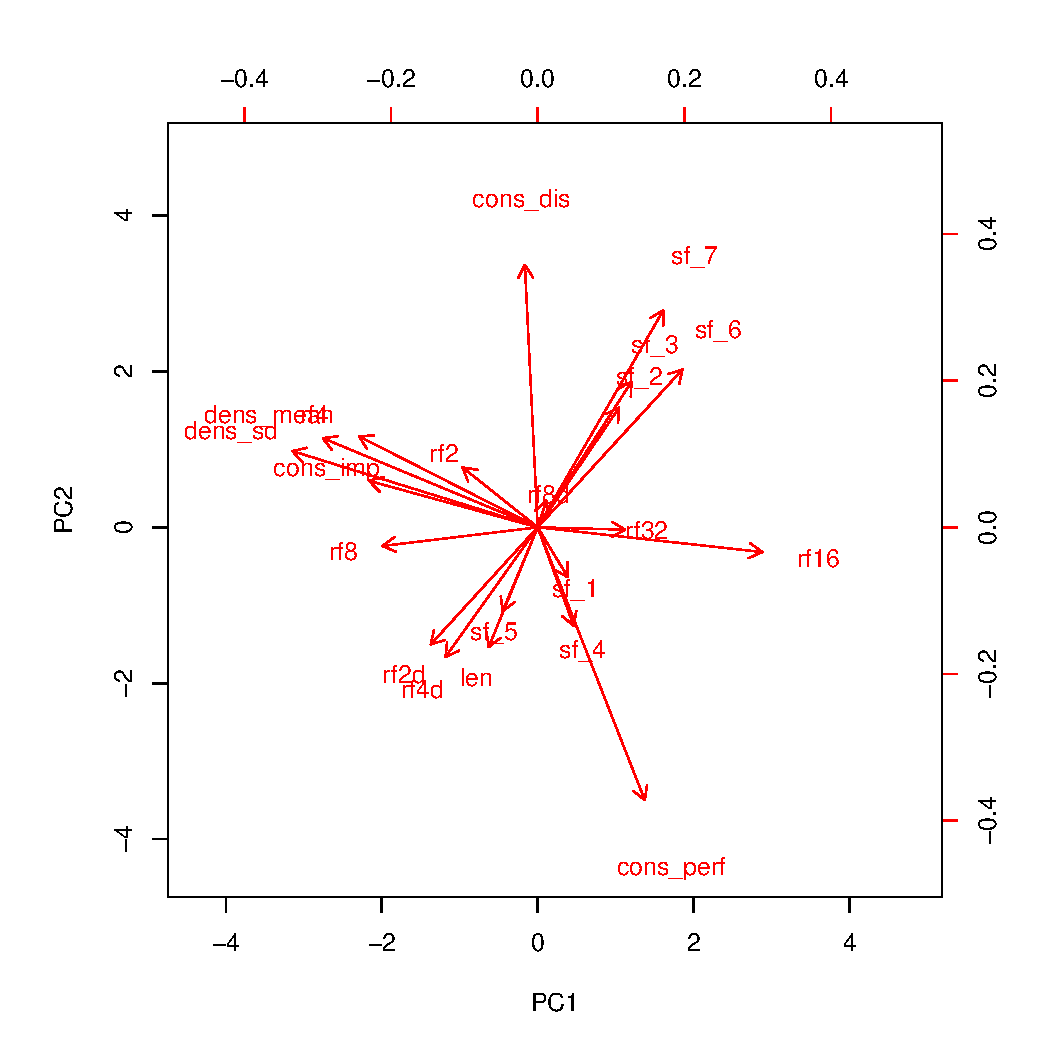
\includegraphics[scale = .7]{images/biplot_b.pdf}
\caption{Biplot of the loading vectors of the first two principal components.}
\label{subd}
\end{figure}
The biplot in Figure 5.4 shows the loading vectors plotted on the first
two principal components. The loading vectors of features seem to
arrange into approximately three groups. The features: perfect
consonances of melodic intervals of the voice, frequency of the first
scale degree, frequency of the fourth scale degree are all grouped
together. Similarly, frequencies for the 7th, 6th, 2nd, and 3rd are
grouped together. In addition we have perfect consonances and imperfect
consonances on two sides of the second principal component. It appears
that the first principal component seems to encode tempo/rhythm. Faster
rhythmic notes, like sixteenth notes and thirty second notes have
opposite loadings than slower rhythmic notes. The second principal
component appears to encodes harmonic structure, especially differences
in consonances.
\begin{figure}[H]
\centering
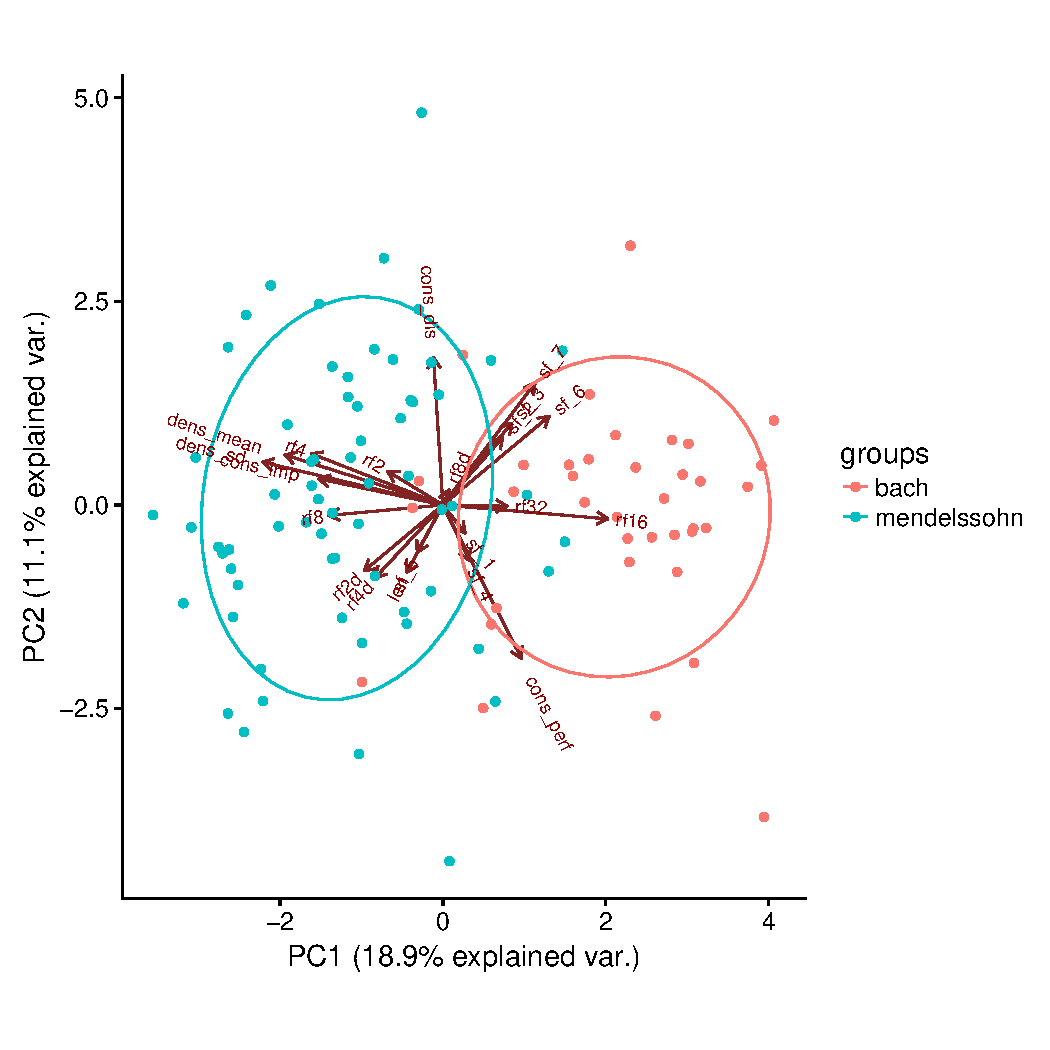
\includegraphics[scale = .7]{images/bi_elipse12.pdf}
\caption{Biplot of the first two principal components plotted with data points colored by composer. }
\label{subd}
\end{figure}
Figure 5.5 shows the same loadings of the principal components, but with
the addition of points representing each piece graphed by their first
two principal components. Each piece is colored by composer. The
ellipses represent a 95\% concentration area, or where 95\% of the data
lie. We can see that the ellipses only overlap slightly, indicating that
pieces by Bach and Mendelssohn usually have different values in the
first and second principal component. Figure 5.6 shows the pieces
plotted on the second and third principal component and there is much
less separation. The third principal component also appears to encode
rhythmic information. We have that dotted rhythmic frequencies have
opposite loadings on the third principal component to their
corresponding non dotted rhythm. For example, frequencies of eight notes
have an opposite loading on the third principal component to the
frequency of dotted eighth notes.
\begin{figure}[H]
\centering
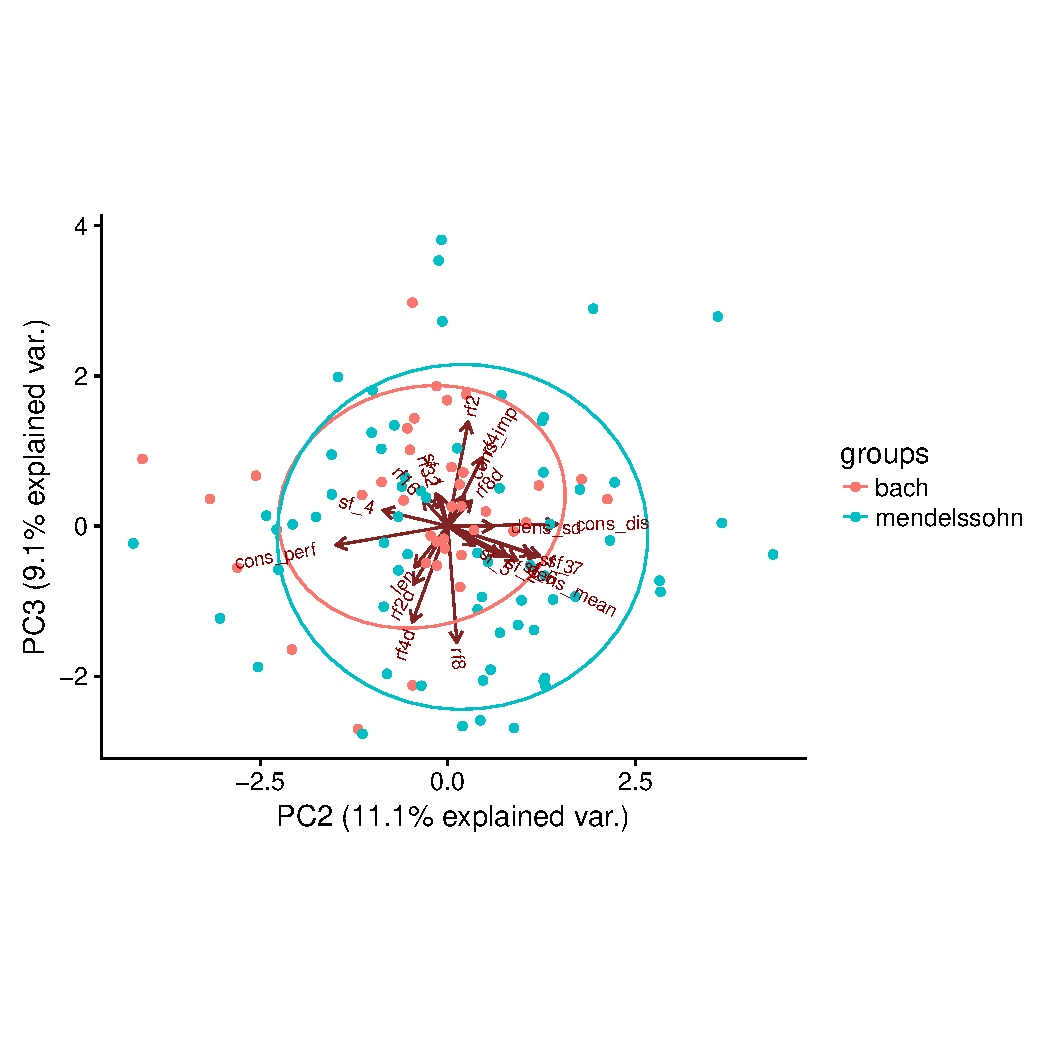
\includegraphics[scale = .7]{images/bi_elipse23.pdf}
\caption{Biplot of the second and third principal components plotted with data points colored by composer.}
\label{subd}
\end{figure}
We can also use K-means clustering to see if there are any apparent
groups in the data. When we run K-means on the first 11 principal
components of Bach and Mendelssohn with K = 2 (since we are comparing
two classes ), we get the results we see in Figure 5.7. The coloring of
the points indicate which cluster the K-means algorithm assigned to each
piece. The label of each piece indicates the actual composer. We can see
that for the most part, for pieces with high or low scores on the first
principal component, the clustering preserves the composer. For pieces
with middle scores of the first PC, there is a good number of pieces
with a cluster assignment not consistent with composer.
\begin{figure}[H]
\centering
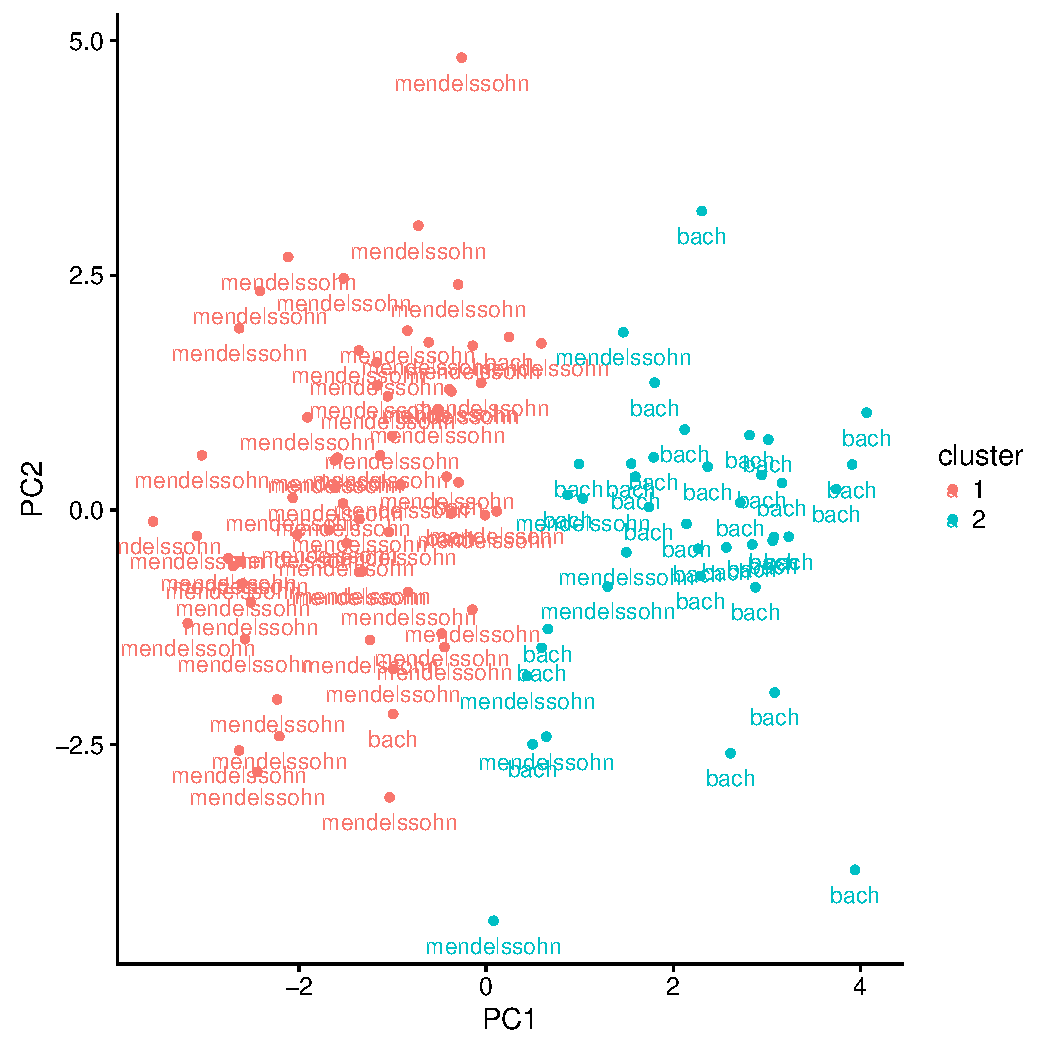
\includegraphics[scale = .7]{images/kmeans_2_b.pdf}
\caption{KNN when k = 2.}
\label{subd}
\end{figure}
We can also examine when \(K=3\), indicating that the \(K-\)means
algorithm should look for three clusters. This is reasonable as the
Mendelssohn set is made up of Fanny and Felix, so there are actually
three composers. The clusters seem to be mostly assigned by the value of
the first principal component. For the most part, pieces by Bach are
assigned to the third cluster, although there are a couple in the other
two clusters.
\begin{figure}[H]
\centering
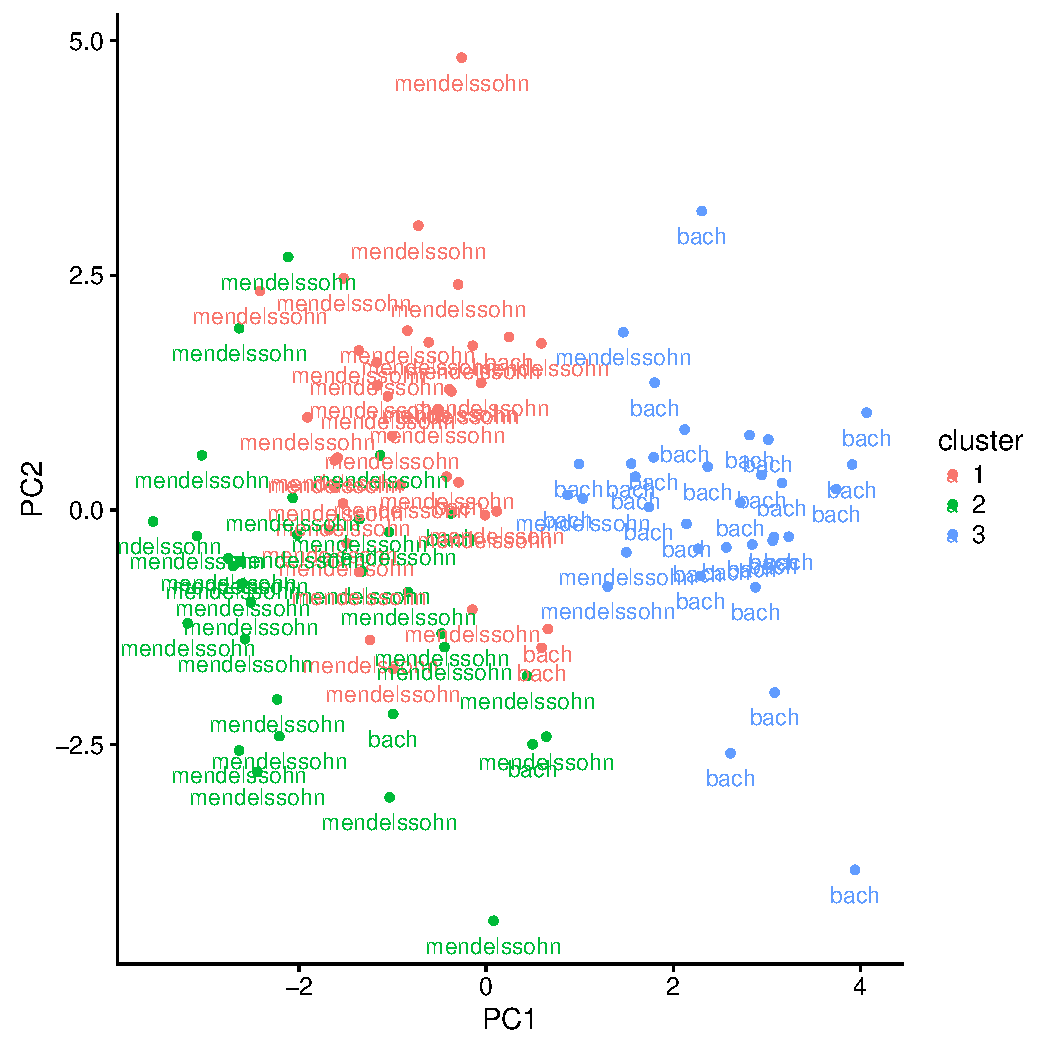
\includegraphics[scale = .7]{images/kmeans_3_b.pdf}
\caption{KNN when $k = 3$.}
\label{subd}
\end{figure}
\section{Felix and Fanny}\label{felix-and-fanny}

As we can see from density distributions in Figure 5.9, most of the
features used have very little separation between the two composers.
Most of the density distributions for features from pieces of Fanny and
Felix overlap completely and have nearly identical peaks. There is a
small difference in peak for the frequency of use of the first scale
degree, with fanny using it more often. The lack of difference in
features between the two composers is not very encouraging for later
fitting of models.
\begin{figure}[H]
\centering
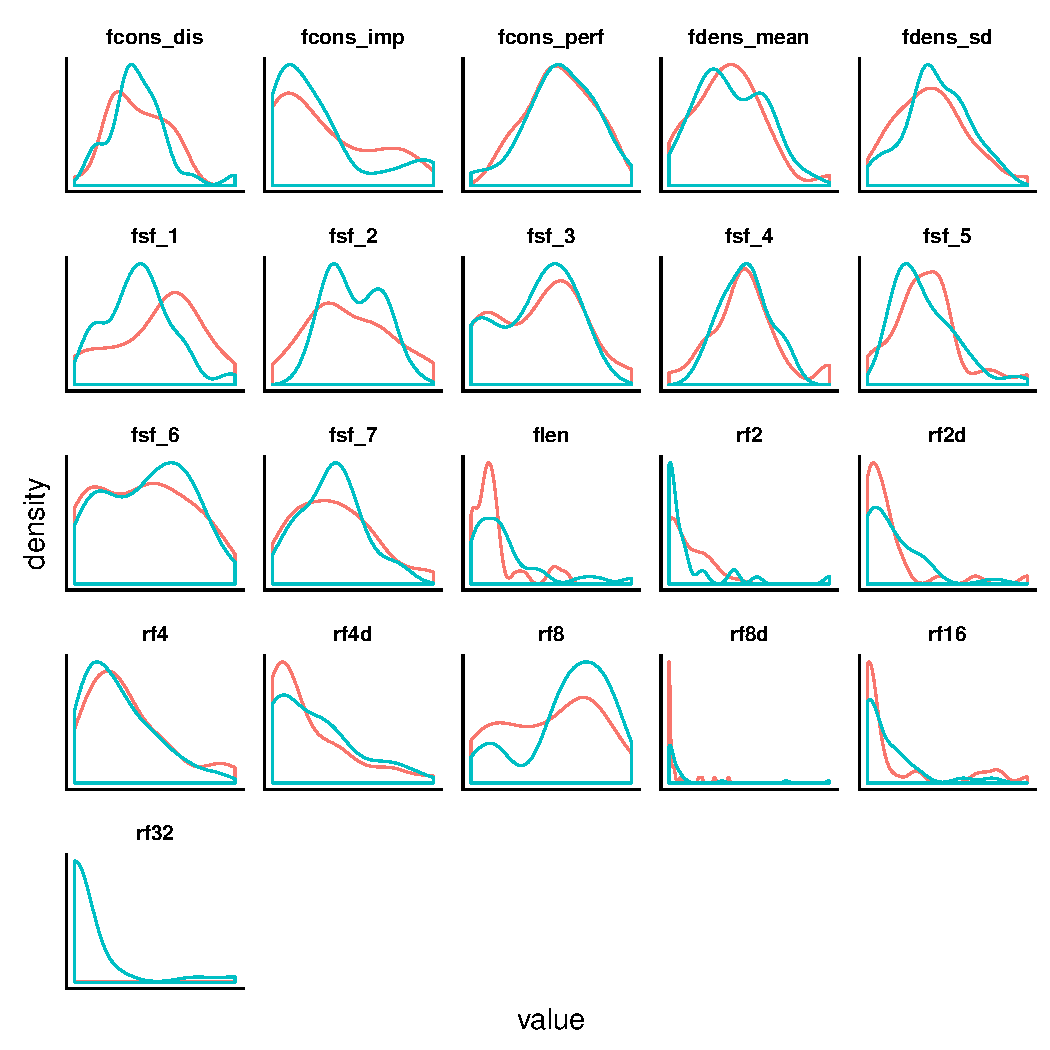
\includegraphics[scale = .7]{images/distribution_f.pdf}
\caption{Density plot of each feature of Fanny/Felix. Blue represents Fanny and red represents Felix.}
\label{subd}
\end{figure}
The correlations of the Fanny/Felix features are shown in Figure 5.10.
The rhythmic features do not seem to have as much correlation as the
Bach/Mendelssohn features. We still see higher correlations for
frequencies of types of melodic consonances, and frequencies of scale
degrees 2, 3, 6, and 7.
\begin{figure}[H]
\centering
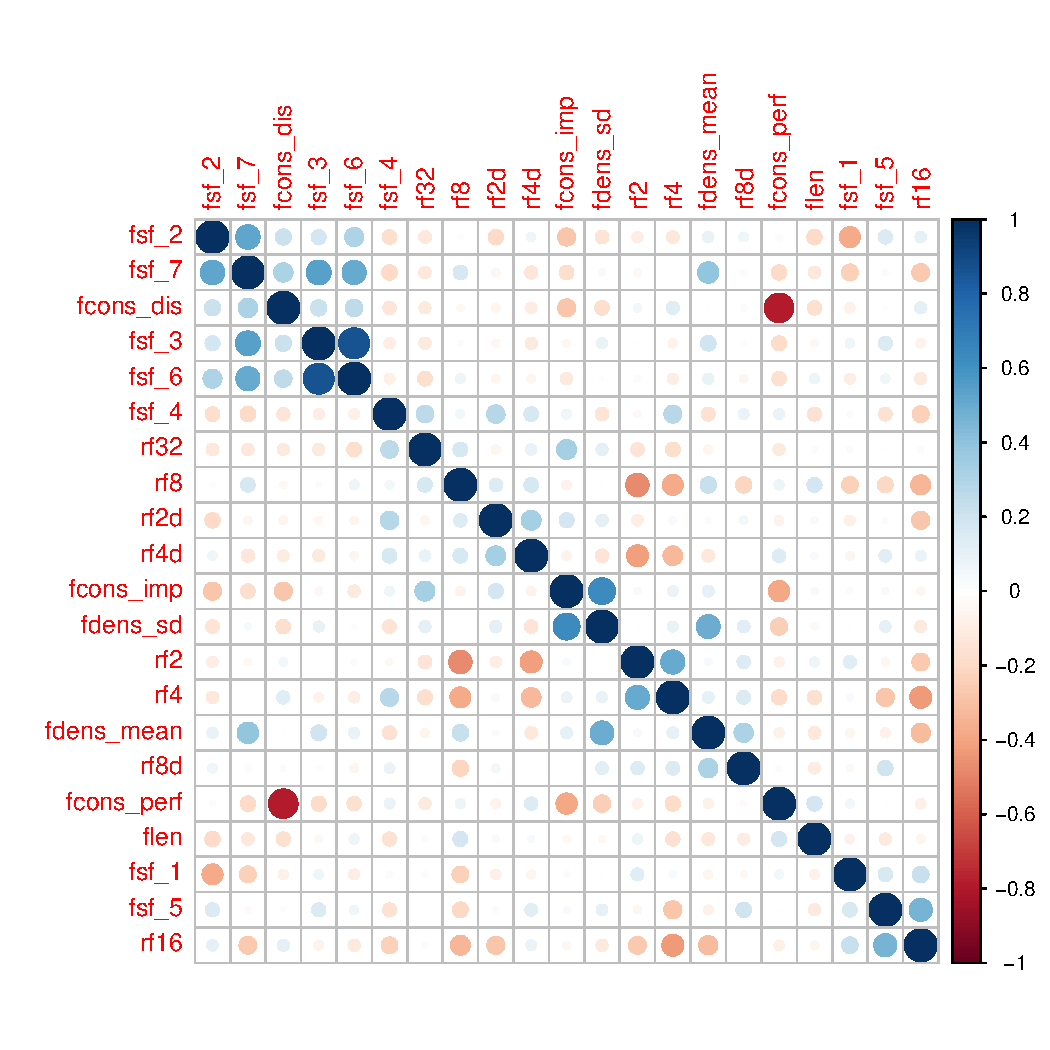
\includegraphics[scale = .7]{images/cor_circles_f.pdf}
\caption{Correlations between features of Fanny/Felix.}
\label{subd}
\end{figure}
Figure 5.11 shows the skree plot for Fanny/Felix. It can be argued that
there is an elbow at principal component thirteen, but it is not that
clear. Using 11 principal components again accounts for 85\% of the
variance, so we will use 11 PCs in fitting our classifiers as well.
\begin{figure}[H]
\centering
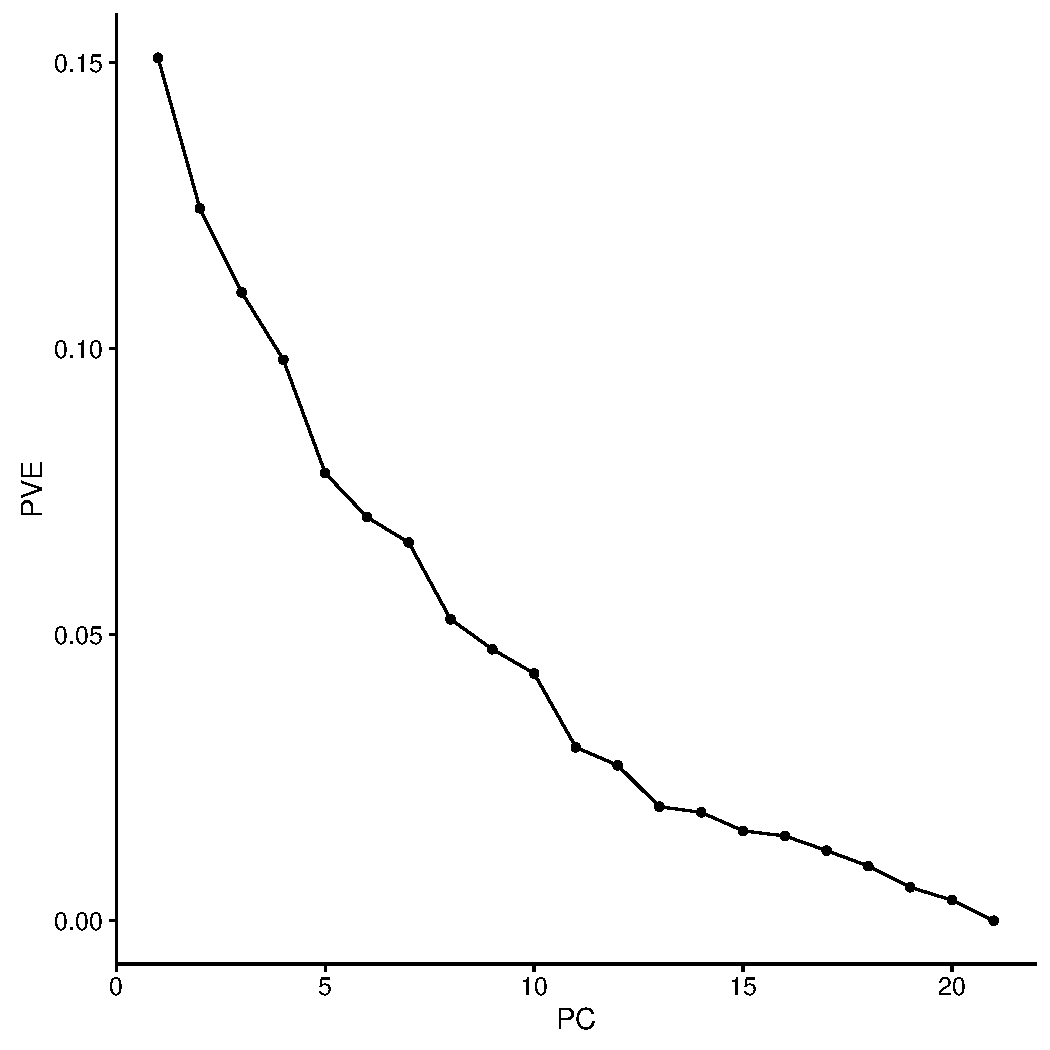
\includegraphics[scale = .7]{images/skree_f.pdf}
\caption{PCA Felix/Fanny skree plot.}
\label{subd}
\end{figure}
\begin{figure}[H]
\centering
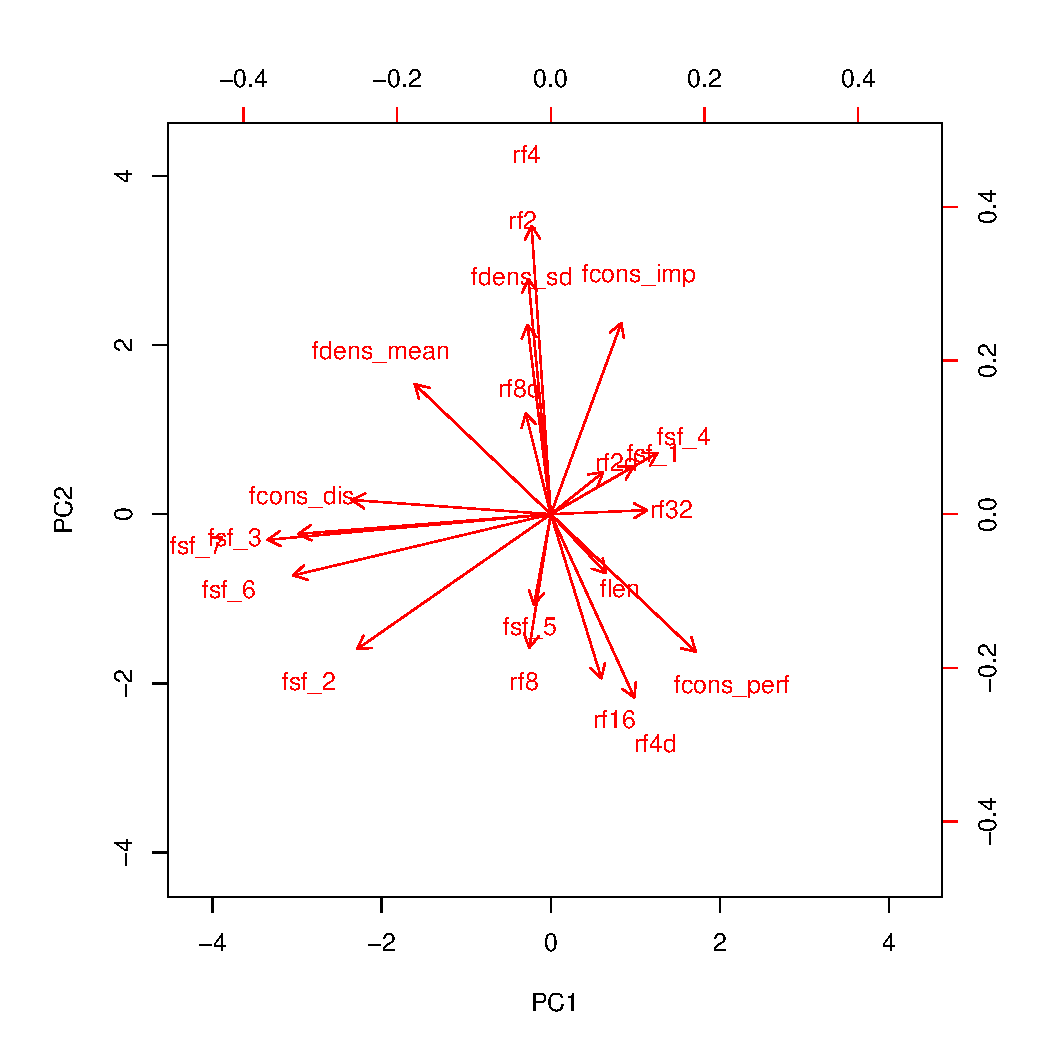
\includegraphics[scale = .7]{images/biplot_f.pdf}
\caption{PCA Loadings of the features for Fanny/Felix.}
\label{subd}
\end{figure}
Figure 5.12 shows the loadings of the principal components of the
features of Fanny and Felix. In contrast to the biplot for
Bach/Mendelssohn, it seems like the first principal component encodes
harmonic aspects of music, and second principal component encodes
rhythm. The loadings for scale degrees 1, 5 and perfect consonant
intervals are in opposite direction on the second principal component to
scale degrees 2, 7 and dissonant intervals. Also we see that frequencies
for faster rhythmic values have opposite loadings to those of slower
notes on the second principal component.
\begin{figure}[H]
\centering
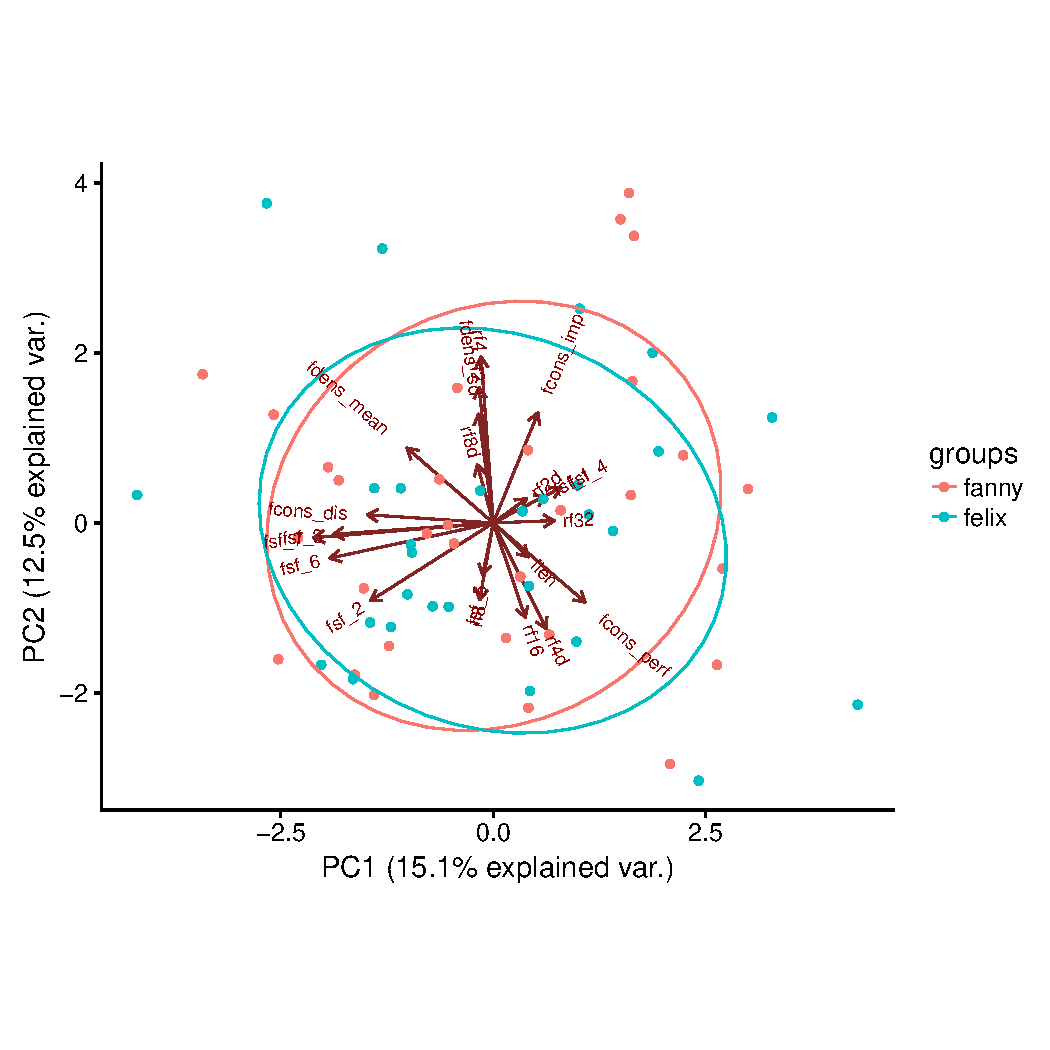
\includegraphics[scale = .7]{images/bi_elipse_12_f.pdf}
\caption{Loadings and pieces for Fanny/Felix.}
\label{subd}
\end{figure}
When the pieces colored by composer are plotted on the biplot as shown
in Figure 5.13, we do not see as much separation between the Fanny and
Felix pieces as how we did for Bach/Mendelssohn. The 95\% ellipses
almost completely overlap. This lack of separation for the two groups
might lead to issues in creating a model to classify.
\begin{figure}[H]
\centering
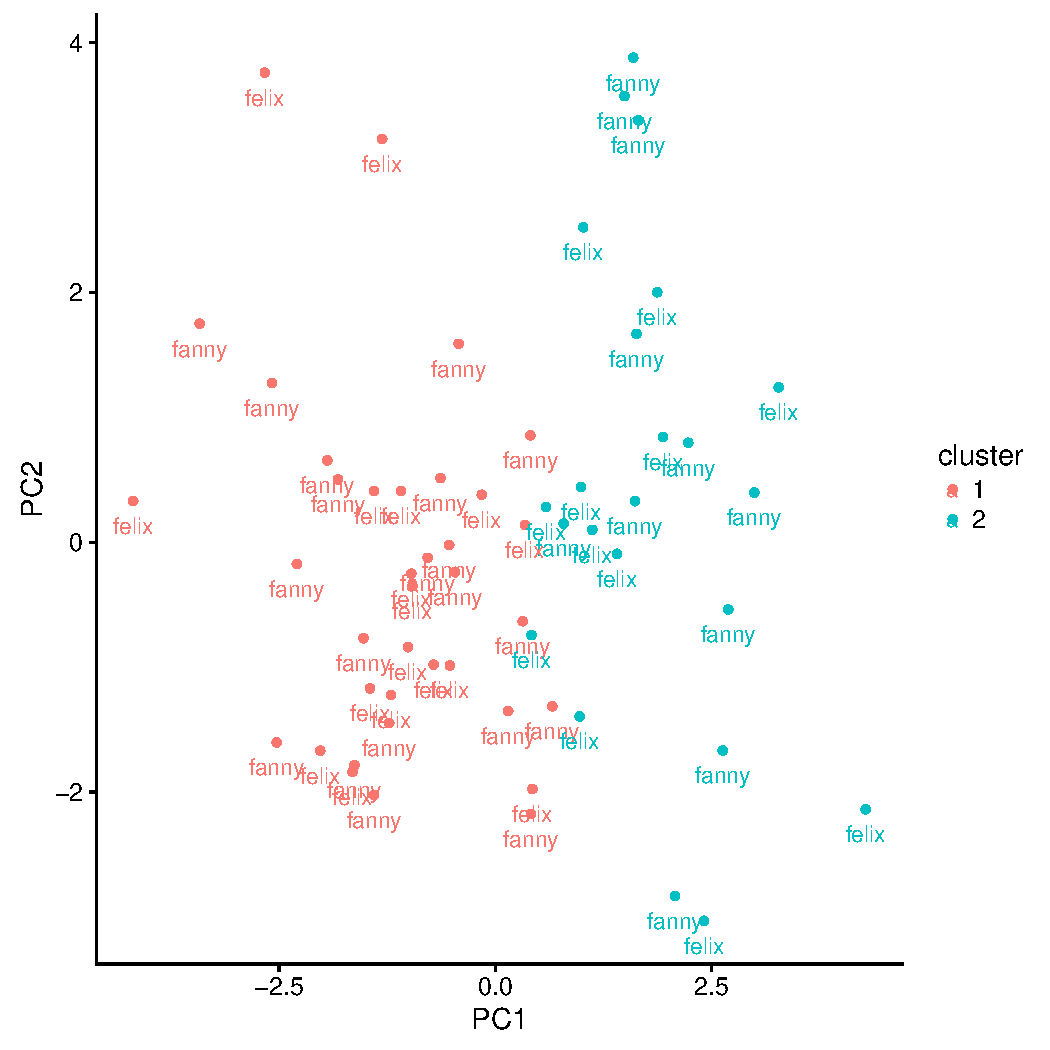
\includegraphics[scale = .7]{images/kmeans_2_f.pdf}
\caption{K-means with k = 2.}
\label{subd}
\end{figure}
We again run \(K-\)means to identify clusters in the data. Ideally,
pieces would be clustered if they shared the same composer, even though
the \(K-\)means algorithm does not have access to the composer
information. Figure 5.14 shows the results of K-means with \(K = 2\). We
see that in the two clusters, there are many pieces labeled of both
composer. This indicates that when clusters that exist in the data, they
do not correspond naturally to composer identification.

\chapter{Classification Results}\label{classification-results}

The following section presents the results of fitting five different
models for classficiation on the original feature space as well as the
first 11 principal components to account for 85\% of the variance. This
was done as there are many features that measure aspects of the same
thing, i.e.~there are seven different features measuring aspects of
scale degree use where each scale degree can individually have
interesting musical interpretations.

The five classifiers were chosen as they were used previously in the
literature for similar problems (KNN, Naive Bayes and Random forests),
or are popular models for classification (Logistic, LDA). For the
logistic classifier we used lasso as a shrinkage method.

Each model (10 total) was tested for predictive accuracy by finding the
\(5-\)fold cross-validated misclassification rate. The cross-validated
misclassification rate showed high of variance depending on the random
fold assigned, so the process was repeated 100 times, and the rate was
averaged.

\section{Models Results -
Bach/Mendelssohn}\label{models-results---bachmendelssohn}
\begin{longtable}[]{@{}lll@{}}
\caption{Averaged 5-fold CV misclassification rates for each model from
100 runs on the feature space and the first 11 PCs.}\tabularnewline
\toprule
Model & misclass. rate - features & misclass. rate - 11
PCs\tabularnewline
\midrule
\endfirsthead
\toprule
Model & misclass. rate - features & misclass. rate - 11
PCs\tabularnewline
\midrule
\endhead
Logistic & 0.078 & 0.097\tabularnewline
LDA & 0.092 & 0.049\tabularnewline
KNN (K = 9) & 0.097 & 0.098\tabularnewline
Naive Bayes & 0.103 & 0.112\tabularnewline
Random forest & 0.058 & 0.111\tabularnewline
\bottomrule
\end{longtable}
Table 6.1 shows the averaged 5-fold cross-validated misclassification
rates over 100 runs. For the KNN case, the features were scaled and
centered first. Most models have misclassification rates round 10\%. The
best model was found to be linear discriminant analysis run on the
principal components.

Figure 6.1 shows coefficient values for each feature for varying
\(\log(\lambda)\) values. \(\lambda\) corresponds to the restriction
penalty. Higher values of \(\log(\lambda)\) correspond to a higher
penalty, resulting in coefficient estimates that shrink to zero. The
cross-validated lasso logistic fit chose \(\log(\lambda) = -6.2\) to
have the lowest misclassification rate. At that value, most features
besides the third and fifth scale degrees and frequency of eighth note
are non-zero. We have that scale degree two and mean density features
have low coefficient estimates at this point, but are non-zero. Overall,
for all \(\lambda\) penalties, it appears that the features for density
and frequency of 16th note rhythms stay non-zero the longest, implying
these features are more useful features for distinguishing the composer.
\begin{figure}[H]
\centering
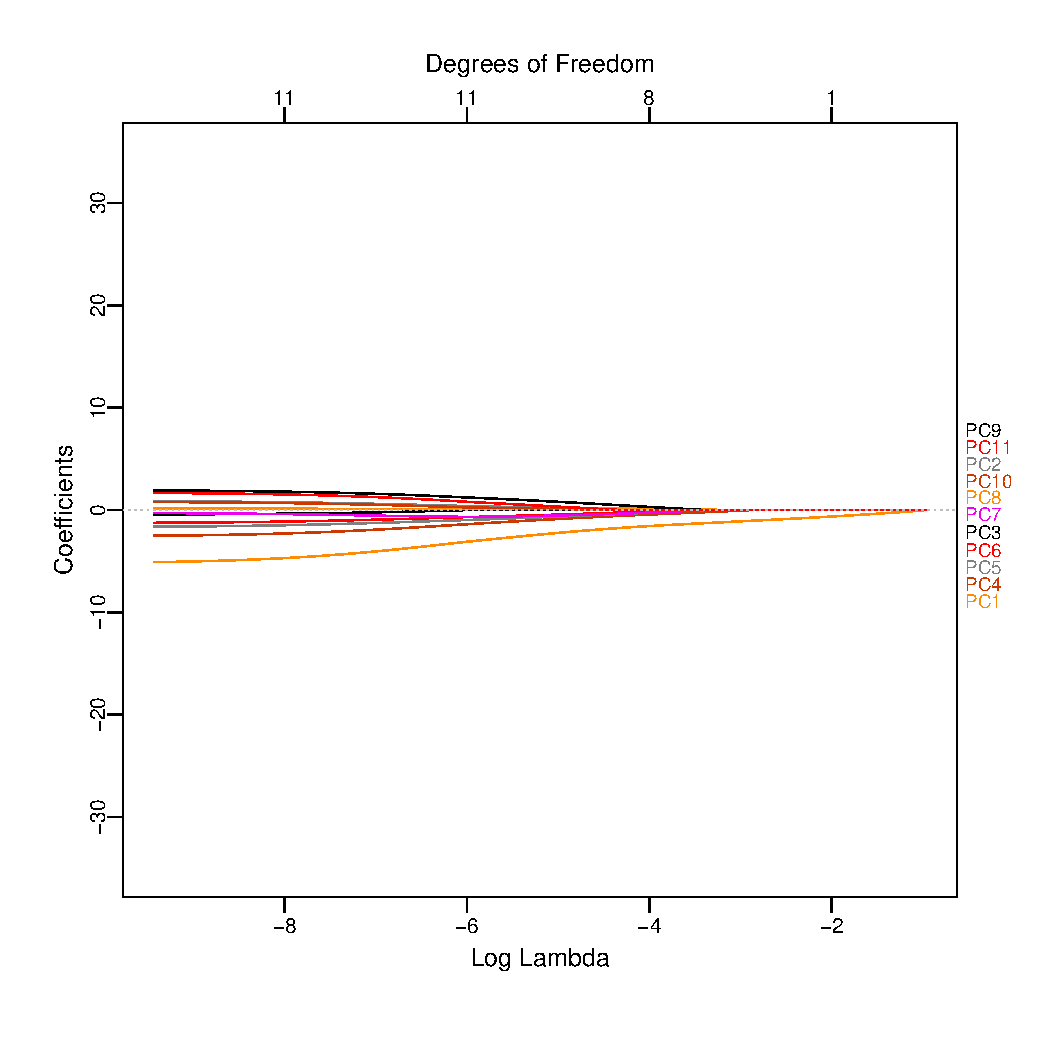
\includegraphics[scale = .6]{images/lasso_coef_b.pdf}
\caption{Bach/Mendelssohn lasso logistic regression coefficients for changing $\lambda$ penalty values. The vertical line represents the value of best $\lambda$.}
\label{subd}
\end{figure}
\begin{figure}[H]
\centering
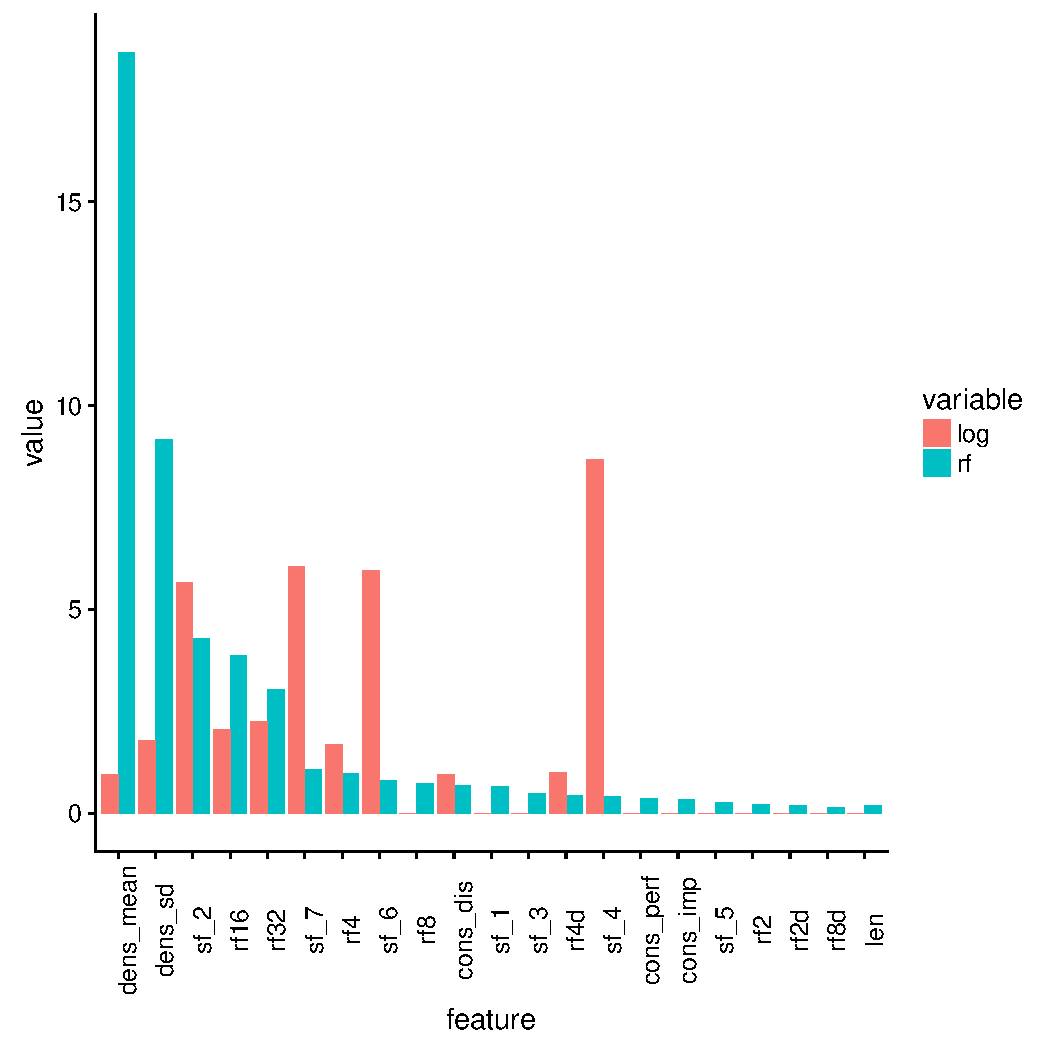
\includegraphics[scale = .5]{images/var_imp_rflog_b.pdf}
\caption{Random forest variable importance and logistic regression coefficients and best $\lambda$ Bach/Mendelssohn.}
\label{subd}
\end{figure}
Figure 6.2 shows the variable importance rankings as a mean decrease in
the Gini index for the random forest model. It also shows the absolute
value of the logistic regression coefficients at the best value for
\(\lambda\). Note that we look at the relative height of the bars here
to determine importance. We can see that while the random forest does
not view frequencies of dotted quarter notes to be a very useful
predictor, the logistic model views it as very important. The density
features are the most important in deciding splits of the trees,
although these values do not have high coefficients in the logistic.
Both models agree that the last seven variables are not important. They
were shrunk to zero in the logistic lasso model.

\section{Model fit Felix/Fanny}\label{model-fit-felixfanny}
\begin{longtable}[]{@{}lll@{}}
\caption{Averaged 5-fold CV misclassification rates of 100 runs on the
feature space and the first 11 principal components for each
model.}\tabularnewline
\toprule
Model & misclass. rate - features & avg. misclass. rate - 11
PCs\tabularnewline
\midrule
\endfirsthead
\toprule
Model & misclass. rate - features & avg. misclass. rate - 11
PCs\tabularnewline
\midrule
\endhead
Logistic & 0.467 & 0.45\tabularnewline
LDA & 0.518 & 0.505\tabularnewline
KNN & 0.498 & 0.467\tabularnewline
Naive Bayes & 0.502 & 0.521\tabularnewline
Random forest & 0.535 & 0.571\tabularnewline
\bottomrule
\end{longtable}
Table 6.2 shows all the misclassification rates of each model. Most of
the misclassification rates are above 0.5, indicating that random
guessing would perform better at predicting the composer. A logistic
lasso classification model fit on the principal components performed
best, with a misclassification rate of 0.45.
\begin{figure}[H]
\centering
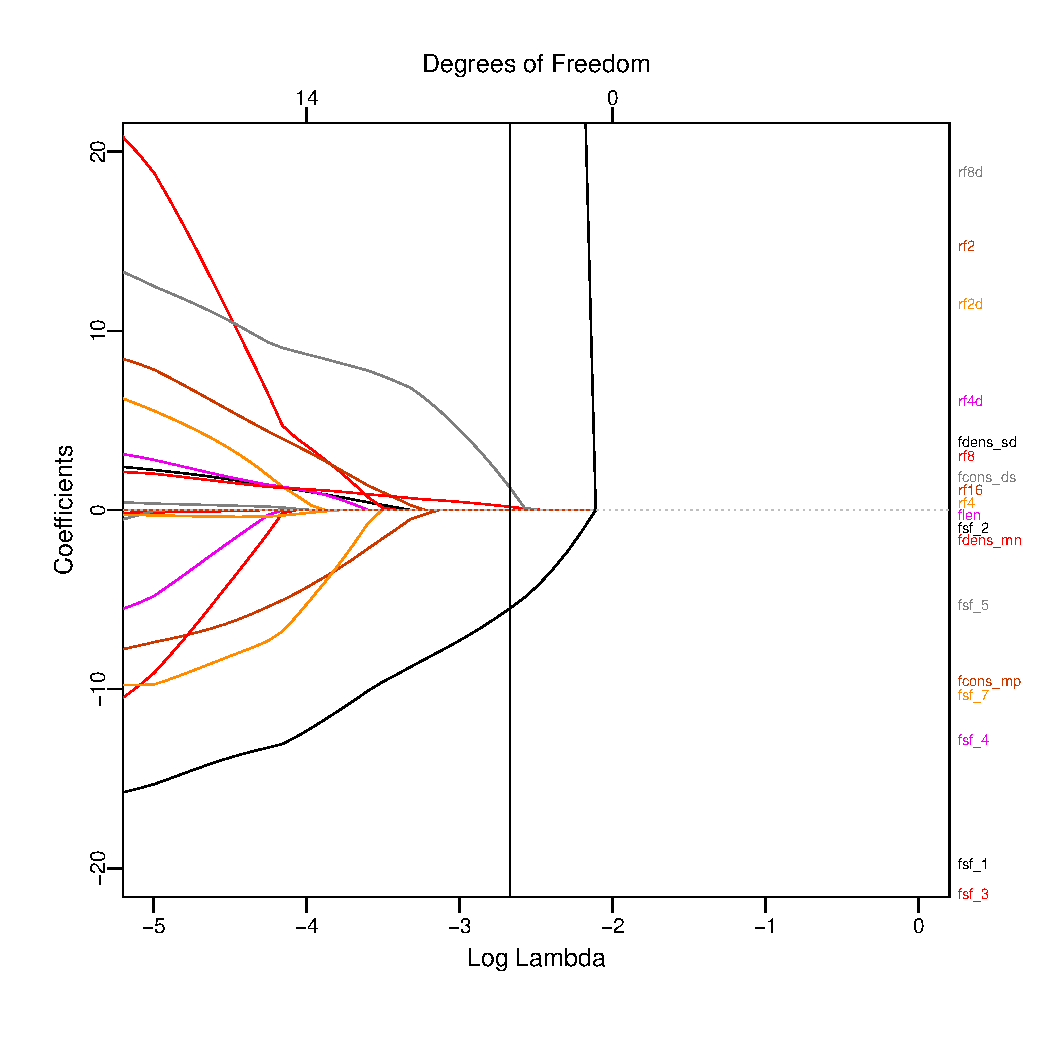
\includegraphics[scale = .6]{images/loglambda_f.pdf}
\caption{Fanny/Felix lasso logistic regression coefficients for changing $\lambda$ penalty values. The vertical line represents the value of best $\lambda$.}
\label{subd}
\end{figure}
Figure 6.3 shows the coefficient estimates for varying \(\log(\lambda)\)
penalties for a logistic lasso model fit on the feature space. The
frequency of the first scale degree appears to remain non-zero for the
longest time. At \(\log(\lambda)\) of -2.67 we get the best \(\lambda\)
fit. At this \(\log(\lambda)\) value we have most of the coefficients
shunk to zero besides frequency of thirty second notes and dotted eighth
notes, and frequency of the tonic (first scale degree).
\begin{figure}[H]
\centering
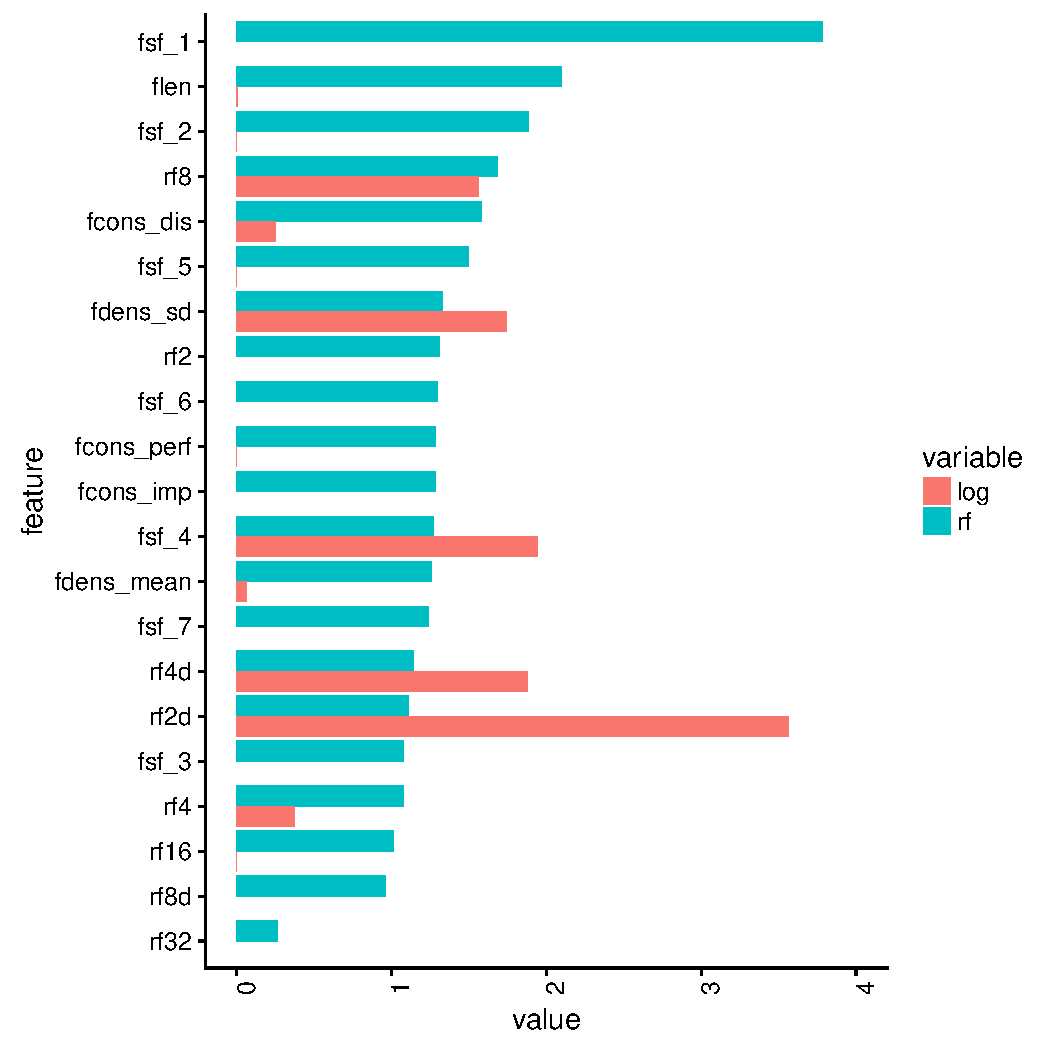
\includegraphics[scale = .5]{images/var_imp_rflog_f.pdf}
\caption{Random forest variable importance and logistic regression coefficients and best $\lambda$ Fanny/Felix.}
\label{subd}
\end{figure}
Figure 6.4 shows the variable importance used in random forests and the
logistic regression coefficients at the best \(\lambda\) value (-2.67).
At the best \(\lambda\) value, only nine of the coefficients of logistic
regression are non-zero. The features that the random forest model found
useful did not correspond very well to the features remaining non-zero
in the logistic lasso model.

\section{Predictions for disputed
pieces}\label{predictions-for-disputed-pieces}

Since we have such high misclassification rates using each model, the
following predictions are likely not accurate. Even so, we do see that
most of the pieces have a higher proportion of predictions for Fanny
than Felix. Table 6.3 shows the predicted classification for each piece
for each model.
\begin{longtable}[]{@{}lllllll@{}}
\caption{Predicted composer for each disputed piece}\tabularnewline
\toprule
Model & Op.8 2 & Op.8 3 & Op.8 12 & Op.9 7 & Op.9 10 & Op.9
12\tabularnewline
\midrule
\endfirsthead
\toprule
Model & Op.8 2 & Op.8 3 & Op.8 12 & Op.9 7 & Op.9 10 & Op.9
12\tabularnewline
\midrule
\endhead
logistic-lasso & fanny & fanny & felix & fanny & felix &
fanny\tabularnewline
LDA & fanny & fanny & fanny & felix & felix & fanny\tabularnewline
KNN & felix & fanny & felix & felix & fanny & felix\tabularnewline
Naive Bayes & fanny & fanny & fanny & fanny & fanny &
fanny\tabularnewline
Random Forest & felix & felix & felix & fanny & fanny &
felix\tabularnewline
\bottomrule
\end{longtable}
\section{Discussion}\label{discussion}

On very basic low-level features, consisting mostly of frequencies of
notes, intervals and chords, most models comparing Bach to the
Mendelssohns do relatively well. This is likely due to the decent
separation of the features encoding density. We likely see so much
separation because the Bach data are for solo piano and the Mendelssohn
data have an additional instrument, thus making the piece automatically
more dense.

On the other hand, models fit to compare Felix and Fanny did not do as
well. They are only very slightly better than random guessing. This
could be because there is no true difference between Fanny and Felix in
the features we extracted, i.e., the features extracted are not good
enough to pick up any existing signal. On the other hand, it is
certainly believable that Fanny and Felix could have very similar
unconscious signals in their writing. They were trained together, and
did critique each others work extensively. The other possibility is that
there are more pieces by Fanny snuck into Felix's published work,
leading to overlap in the extracted features. These features did
accurately predict composer for the previous comparison
(Bach/Mendelssohn), but perhaps composers so similar in style cannot be
differentiated using these features. The included features only encode
very basic aspects of music, and are more based on frequencies than how
music actually seems to differ in style to a listener, such as features
for uses of melodic phrasing.

Running the classfication models on the first eleven principal
components resulted in a slight improvement for two of the models in the
Bach/Mendelssohn comparison, and a slight improvement for three of the
models in the Fanny/Felix comparison. For LDA, at least, we know LDA is
a model that is sensitive to collinearity, and running on the principal
components helps with this. For the models where no improvement was made
using the principal components, it is possible that those models did
better with more information included. Perhaps we should have chosen
more principal components to account for more explanation of variance to
be used in models.

Even though our classifiers for Felix/Fanny did not perform very well,
it does seem like there is a good amount of musical interpretation
contained in the features used. The first three principal components of
the features seem to correspond to harmonic meaning, rhythmic meaning,
and dotted vs not dotted notes.

\chapter*{Conclusion}\label{conclusion}
\addcontentsline{toc}{chapter}{Conclusion}

Fitting classifiers using low-level features composed mostly of
frequencies of notes and rhythms was able to differentiate style between
Bach and Fanny and Felix Mendelssohn. However classifiers using these
low-level features were not successful in differentiating between Fanny
and Felix. Of the ten models fit on pieces by Fanny and Felix, only 4/10
did better than random guessing. The \(k-\)nearest neighbor classifier
and lasso logistic performed the best. Thus the low-level features used
in this study were not able to measure style differences between Fanny
and Felix. This is likely either to the fact that these features were
not able to pick an existing signal, or that Fanny and Felix have no
discernible difference in style, although the first is more likely. Most
of the previous studies regarding composer identification were able to
distinguish composer. The work by Brinkman when comparing Josquin to
contemporaries did have substantial error in assigning composers
although not as bad as our classifiers performed, except for de Orto.
Josquin and his contemporaries however, did not grow up together or
receive identical music training, like Fanny and Felix did. Also
analyzing music in the Romantic era has not been done before, and
perhaps different kinds of features need to be created to train a
successful classifier.

\section{Future suggestions for research and expansion of
museR}\label{future-suggestions-for-research-and-expansion-of-muser}

Most suggestions for future work lie in expanding the capabilities for
museR. One issue to be improved upon is increasing the ease of importing
data. The scanning/OMR step is incredibly time consuming, which lead to
a limited number of pieces being used in this analysis. Running this
same analysis with more data could also lead to better results and lower
errors, or at least errors with smaller variance. While museR cannot
directly help with speeding up the scanning process, museR could be
expanded to be able to import music in the musicXML format in order to
not need to rely on Humdrum's conversion program. Future versions of
museR will ideally be able to extract high level features. These are
features that take into account the context of the music from where the
feature is extracted. These features could include more harmonic
features, such as chord progressions, and more chord analysis. These
high level features are what humans generally pick up on when
distinguishing style. In addition, in the future, museR should be able
to implement windowing techniques for extracting features. These
features could still be low-level features, but they might have more
meaning in determining style as they are on a smaller scale instead of
averaged across the entire piece.

In addition, it would be interesting to perform this same analysis on
music of different types of pieces. We might expect unconscious signals
to exist in the same way in symphonies as well as lieder, or perhaps
not. Considering features that are similar between symphonic work and
solo piano works is a challenging problem in of itself. Also, including
another composer in this study, perhaps a contemporary of Felix and
Fanny, or at least a composer in the Romantic era would also be helpful
in checking the validity of the features. Also, it would be interesting
to examine composers throughout their career. Composers, Dvorak for
example, changed drastically their career. Maybe composers have
different aspects of style when they first started composing than when
they were older. Ideally, museR could be used to pick up on these
differences.

\chapter*{Appendix}\label{appendix}
\addcontentsline{toc}{chapter}{Appendix}

\section*{How to download museR}\label{how-to-download-muser}
\addcontentsline{toc}{section}{How to download museR}

The following commands download \texttt{museR} from GitHub.
\begin{Shaded}
\begin{Highlighting}[]
\KeywordTok{library}\NormalTok{(devtools)}
\KeywordTok{install_github}\NormalTok{(}\StringTok{"empalmer/Thesis/museR"}\NormalTok{)}
\end{Highlighting}
\end{Shaded}
\backmatter

\chapter*{References}\label{references}
\addcontentsline{toc}{chapter}{References}

\markboth{References}{References}

\noindent

\setlength{\parindent}{-0.20in} \setlength{\leftskip}{0.20in}
\setlength{\parskip}{8pt}

\hypertarget{refs}{}
\hypertarget{ref-adair1944}{}
Adair, D. (1944). The authorship of the disputed federalist papers.
\emph{The William and Mary Quarterly: A Magazine of Early American
History,} 98--122.

\hypertarget{ref-harmonicon}{}
Ayrton, W. (1830). \emph{The harmonicon} (Vol. 8). W. Pinnock.

\hypertarget{ref-backer2005}{}
Backer, E., \& Kranenburg, P. van. (2005). On musical stylometry---a
pattern recognition approach. \emph{Pattern Recognition Letters},
\emph{26}(3), 299--309.

\hypertarget{ref-brinkman2016}{}
Brinkman, A., Shanahan, D., \& Sapp, C. (n.d.). Musical stylometry,
machine learning, and attribution studies: A semi-supervised approach to
the works of josquin.

\hypertarget{ref-crerar}{}
Crerar, M. (1985). Elements of a statistical approach to the question of
authorship in music. \emph{Computers and the Humanities}, \emph{19}(3),
175--182.

\hypertarget{ref-OMR}{}
Doermann, D., Tombre, K., \& others. (2014). \emph{Handbook of document
image processing and recognition}. Springer.

\hypertarget{ref-authorshipfed}{}
Ford, P. L., \& Bourne, E. G. (1897). The authorship of the federalist.
\emph{The American Historical Review}, \emph{2}(4), 675--687. Retrieved
from \url{http://www.jstor.org/stable/1833983}

\hypertarget{ref-esl}{}
Friedman, J., Hastie, T., \& Tibshirani, R. (2001). \emph{The elements
of statistical learning} (Vol. 1). Springer series in statistics New
York.

\hypertarget{ref-guyon2003}{}
Guyon, I., \& Elisseeff, A. (2003). An introduction to variable and
feature selection. \emph{Journal of Machine Learning Research},
\emph{3}(Mar), 1157--1182.

\hypertarget{ref-hoer}{}
Hoerl, A. E. (1959). Optimum solution of many variables equations.
\emph{Chemical Engineering Progress}, \emph{55}(11), 69--78.

\hypertarget{ref-huron1994humdrum}{}
Huron, D. (1994). The humdrum toolkit reference manual, ccarh. Stanford
University.

\hypertarget{ref-isl}{}
James, G., Witten, D., Hastie, T., \& Tibshirani, R. (2013). \emph{An
introduction to statistical learning} (Vol. 112). Springer.

\hypertarget{ref-laitz}{}
Laitz, S. G. (2012). \emph{The complete musician: An integrated approach
to tonal theory, analysis, and listening}. Oxford University Press.

\hypertarget{ref-mace2013}{}
Mace, A. R. (2013). \emph{Fanny hensel, felix mendelssohn bartholdy, and
the formation of the`` mendelssohnian'' style} (PhD thesis).

\hypertarget{ref-mearns2010}{}
Mearns, L., Tidhar, D., \& Dixon, S. (2010). Characterisation of
composer style using high-level musical features. In \emph{Proceedings
of 3rd international workshop on machine learning and music} (pp.
37--40). ACM.

\hypertarget{ref-mosteller1964inference}{}
Mosteller, F., \& Wallace, D. (1964). \emph{Inference and disputed
authorship: The federalist}. Addison-Wesley.

\hypertarget{ref-papadopoulosai}{}
Papadopoulos, G., \& Wiggins, G. (n.d.). AI methods for algorithmic
composition: A survey, a critical view and future prospects.

\hypertarget{ref-pudil1994floating}{}
Pudil, P., Novovičová, J., \& Kittler, J. (1994). Floating search
methods in feature selection. \emph{Pattern Recognition Letters},
\emph{15}(11), 1119--1125.

\hypertarget{ref-reich1991}{}
Reich, N. B. (1991). The power of class: Fanny hensel. \emph{Mendelssohn
and His World}, 86--99.

\hypertarget{ref-sapp}{}
Sapp, C. S. (n.d.). CCARH homepage. \emph{CCARH Homepage}. Retrieved
from \url{http://www.ccarh.org/}

\hypertarget{ref-jrp}{}
The josquin research project. (n.d.). \emph{The Josquin Research
Project}. Retrieved from \url{http://josquin.stanford.edu/}

\hypertarget{ref-lasso}{}
Tibshirani, R. (1996). Regression shrinkage and selection via the lasso.
\emph{Journal of the Royal Statistical Society. Series B
(Methodological)}, 267--288.

\hypertarget{ref-tillard1996}{}
Tillard, F. (1996). \emph{Fanny mendelssohn}. Hal Leonard Corporation.

\hypertarget{ref-todd2003}{}
Todd, R. L. (2003). \emph{Mendelssohn: A life in music}. Oxford
University Press.

\hypertarget{ref-ldadim}{}
Ye, J., Janardan, R., \& Li, Q. (2005). Two-dimensional linear
discriminant analysis. In \emph{Advances in neural information
processing systems} (pp. 1569--1576).


% Index?

\end{document}
